\documentclass[11pt]{article}
\usepackage{hyperref}
\usepackage{amsmath, amsfonts, amssymb, mathrsfs, dsfont}
\usepackage{dcolumn}
\usepackage{caption}
\usepackage{subcaption}
\usepackage{filemod}
\usepackage{natbib}
\usepackage[ruled, vlined]{algorithm2e}
\usepackage{floatrow}
\usepackage{setspace}
\usepackage{verbatim}
\usepackage{graphicx}
\usepackage{bbm} % for indicator function
\usepackage{xcolor} % only for coloring text while revising

\hypersetup{
    colorlinks=true,
    linkcolor=blue, 
    urlcolor=black,
    citecolor=blue, 
    }

\oddsidemargin=0.25in
\evensidemargin=0.25in
\textwidth=7in
\textheight=8.75in
\topmargin=-.5in
\addtolength{\oddsidemargin}{-.5in}
\addtolength{\evensidemargin}{-.5in}
\footskip=0.5in
%\doublespacing

\title{Bayesian Deep Gaussian Processes for Correlated Functional Data: \\
        A Case Study in Cosmological Power Spectra}
\author{Stephen A. Walsh\thanks{Corresponding author: Division of Natural Sciences, 
        Math and Technology, Elms College, {\tt walshst@elms.edu}} \and 
        Annie S. Booth\thanks{Department of Statistics, Virginia Tech} \and
        David Higdon\footnotemark[2] \and
        Marco A.R. Ferreira\footnotemark[2] \and
        Jared Clark\footnotemark[2] \and
        Kelly Moran\thanks{Los Alamos National Laboratory} \and
        Katrin Heitmann\thanks{Argonne National Laboratory}}
\date{\today}


\begin{document}

\maketitle
\bigskip

\begin{abstract} 
Understanding the structure of our universe and the distribution of matter is an 
area of active research.  As cosmological surveys grow in complexity, the development 
of emulators to efficiently and effectively predict matter power spectra is essential.  
We are particularly motivated by the Mira-Titan Universe simulation
suite which, for a specified cosmological parameterization (termed a ``cosmology''), 
provides multiple response curves of various fidelities, including correlated 
functional realizations.  Our objective is two-fold.  First, we estimate 
the underlying true matter power spectra, with appropriate uncertainty 
quantification (UQ), from all of the provided curves.  To this end, we propose a 
novel Bayesian deep Gaussian process (DGP) hierarchical model which synthesizes 
all the simulation information to estimate the underlying matter power spectra
while providing effective UQ.  Our model extends previous work on Bayesian DGPs 
from scalar responses to correlated functional outputs.  Second, we leverage our predicted 
power spectra from various cosmologies in order to accurately predict the entire 
matter power spectra for an 
unobserved cosmology.  For this task, we use basis function representations 
of the functional spectra to train a separate Gaussian process emulator.  
Our method performs well in synthetic exercises and against the benchmark cosmological 
emulator (Cosmic Emu).
\end{abstract}

\noindent \textbf{Keywords:} computer experiment, Cosmic Emu, 
principal components analysis, Mira-Titan, surrogate, uncertainty quantification

%\vfill

\section{Introduction}
%%%%%%%%%%%%%%%%%%%%%%%%%%%%%%%%%%%%%%%%%%%%%%%%%%%%%%%%%%%%%%%%%%%%%%%%%%%%%%%

%To further our understanding of the structure and movement of the universe, 
%researchers utilize numerous cosmological surveys such as the Sloan Digital Sky 
%Survey \citep{york2000sloan} and the upcoming Nancy Grace Roman Space Telescope 
%\citep{Dore2019WFIRST} which are continuously growing in complexity. With these 
%tools, cosmologists aim to continue learning more about cosmic acceleration 
%\citep{caldwell2009physics}. To this end, one important ingredient to aid in this 
%understanding of our universe is the matter power spectrum. 

Computer simulation experiments are invaluable tools in the study of cosmology.
Experiments which simulate the expansion of the universe are growing
in prevalance and complexity \citep[e.g.,][]{lawrence2010coyote,derose2019aemulus,
nishimichi2019dark,angulo2021bacco,euclid2021euclid,moran2023mira}.  
We are particularly motivated by a simulation
of the matter power spectrum, which describes the distribution of matter as a 
function of spatial scale. 
%It is often represented as a function of wavenumber $k$ (units Mpc$^{-1}$), which is 
%inversely related to spatial scale. 
On large scales, power spectrum behave according to linear perturbation 
theory \citep{pietroni2008flowing, lesgourgues2009non}.  On smaller scales, nonlinear 
dynamics require the use of computationally intensive simulations, yielding
correlated functional data.
%the Coyote Universe \citep{lawrence2010coyote} and the Mira-Titan Universe \citep{moran2023mira} 
%are two simulation suites dedicated to this effort.  
Our overarching goal is to leverage such simulation data to 
first estimate and then predict underlying power matter spectra for various 
cosmological parameterizations.

The Mira-Titan simulation suite \citep{moran2023mira}
defines ``cosmologies'' according to eight cosmological parameters (more on this
in Section \ref{sec:data}).  For a particular cosmology, the simulation of the power matter spectrum 
is rather complex.  Although we presume there exists some true matter spectrum as a function
of wavenumber, we are not able to directly observe it.  Rather, the simulation returns
a convoluted patchwork of potential spectra, which vary in fidelity and are only trusted
over particular wavenumber ranges.  Our first objective is to synthesize expert knowledge
and all available simulation information into an effective estimate of the true underlying
matter spectrum.  

There are several challenges to estimating the underlying spectrum.  Our model
must: handle multiple correlated functional observations, offer enough 
flexibility to accommodate the nonstationarity present in power matter spectra 
(which vary in smoothness across wavenumbers), provide effective uncertainty
quantification (UQ), and allow for the incorporation of expert knowledge 
regarding the wavenumbers over which various outputs are trusted.  To this end, 
we propose a Bayesian hierarchical model which treats functional simulation 
outputs as realizations of a Gaussian process (GP) 
centered on the true underlying spectrum, which itself is a realization of a deep Gaussian process 
\citep[DGP;][]{damianou2013deep}.  The GP accommodates correlated observations
through its covariance structure.  The depth of the DGP offers nonstationary
flexibility.  The Bayesian framework facilitates UQ and the incorporation of prior
knowledge.  While Bayesian DGPs have been previously deployed for computer experiments 
with scalar responses \citep[e.g.,][]{sauer2023active,sauer2023vecchia,ming2023deep}, 
they have yet to be extended to correlated functional outputs. 
To demonstrate the profiency of our Bayesian hierarchical DGP, 
we benchmark its performance in two unique settings: with synthetic data 
mimicing the Mira-Titan data and with real-world data from 
the Code for Anisotropies in the Microwave Background \citep[CAMB;][]{lewis2011CAMB}.
The CAMB model exhibits similar behavior to Mira-Titan but crucially
provides a ``true" power spectrum for each cosmology.

Our second objective is to leverage simulation data from a limited set of
cosmologies in order to predict power matter spectra for unobserved cosmologies.
Due to the computationally expensive nature of the Mira-Titan simulation suite
(one batch of simulations can take multiple weeks to run on a supercomputer),
it is infeasible to evaluate the simulation for every possible eight-dimensional
cosmological configuration which may be of interest.  Instead, we desire
a statistical ``emulator'' or ``surrogate model'' 
\citep{santner2003design,gramacy2020surrogates} which will provide quick and effective
predictions of power matter spectra for any cosmological parameterization.
\citet{moran2023mira} provide a state-of-the-art emulator for the Mira-Titan
simulation suite, which was trained on 117 simulations, and is termed 
the ``Cosmic Emu.''\footnote{\url{https://github.com/lanl/CosmicEmu}}
We leverage the same training data, in conjunction with our Bayesian hierarchical
DGP model and basis function representations, to train a GP surrogate 
on principal component weights in order to predict spectra for unobserved
cosmologies \citep{higdon2008computer, higdon2010estcosmo}. 
Our method compares favorably to Cosmic Emu on held-out cosmologies.

The remainder of the paper is organized as follows.  Section \ref{sec:data} 
introduces our motivating application, the Mira-Titan simulation suite.  
Section \ref{sec:hm_fit} describes our hierarchical Bayesian DGP and 
validates its performance on synthetic exercises and the CAMB simulations.  
Leveraging this trained model, Section \ref{sec:pred} details 
our procedure for predicting at unobserved cosmologies, benchmarking against
state-of-the-art competitors on the CAMB and Mira-Titan simulations. 
Section \ref{sec:disc} concludes with a discussion of our contributions and avenues for 
future research.  We provide reproducible code and an {\sf R} package for our 
Bayesian DGP model in a public git repository.\footnote{\url{https://github.com/stevewalsh124/dgp.hm}}
%\textcolor{cyan}{Please note: this repository is currently private until we 
%hear back regarding permissions for sharing the Mira-Titan data alongside our code.}

%Leveraging these simulations allows for emulation and prediction of the matter power 
%spectrum under varying specifications for eight different cosmological parameters 
%(i.e., different cosmologies). Estimating and understanding the influence of these 
%parameters on cosmic expansion are areas of active research. In addition to 
%presenting the Mira-Titan simulation suite, \cite{moran2023mira} builds off 
%of previous spectrum emulation \citep{lawrence2017mira} to provide the final 
%emulator (Cosmic Emu) based on the full suite of 117 batches of simulations. 

%In this work, we expand on the previous emulation approaches and propose a 
%novel synthesis of methods to quantify uncertainty and predict matter power 
%spectra for different cosmologies using deep Gaussian processes (DGPs). In order 
%to handle multiple realizations of functional output (from the Mira-Titan 
%simulation suite), we use hierarchical modeling and basis functions within our 
%DGP framework to accurately estimate and predict power spectra for different 
%cosmologies. 

\section{Mira-Titan}
\label{sec:data}

The Mira-Titan simulation dataset consists of simulated power spectra for 
117 unique cosmologies. Each of these cosmologies is specified by eight cosmological 
parameters: matter density, baryon density, amplitude of density fluctuations, 
dimensionless Hubble parameter, spectral index of scalar perturbations,
dark energy equation of state parameters, and neutrino density. For more details 
on these parameters and their effects, see \cite{dodelson2020modern, aghanim2020planck, heitmann2016mira}. 
Parameter ranges are specified in Table 2.1 of \cite{moran2023mira}.
There is an optional ninth parameter, the redshift, which we fix at 0.
%Different simulation output exists for different values of a ninth value, 
%the redshift; in this work, we fix 
%this value at 0. 

% after \linewidth:, trim=0 13 0 45, clip=TRUE
\begin{figure}[ht]
    \centering 
    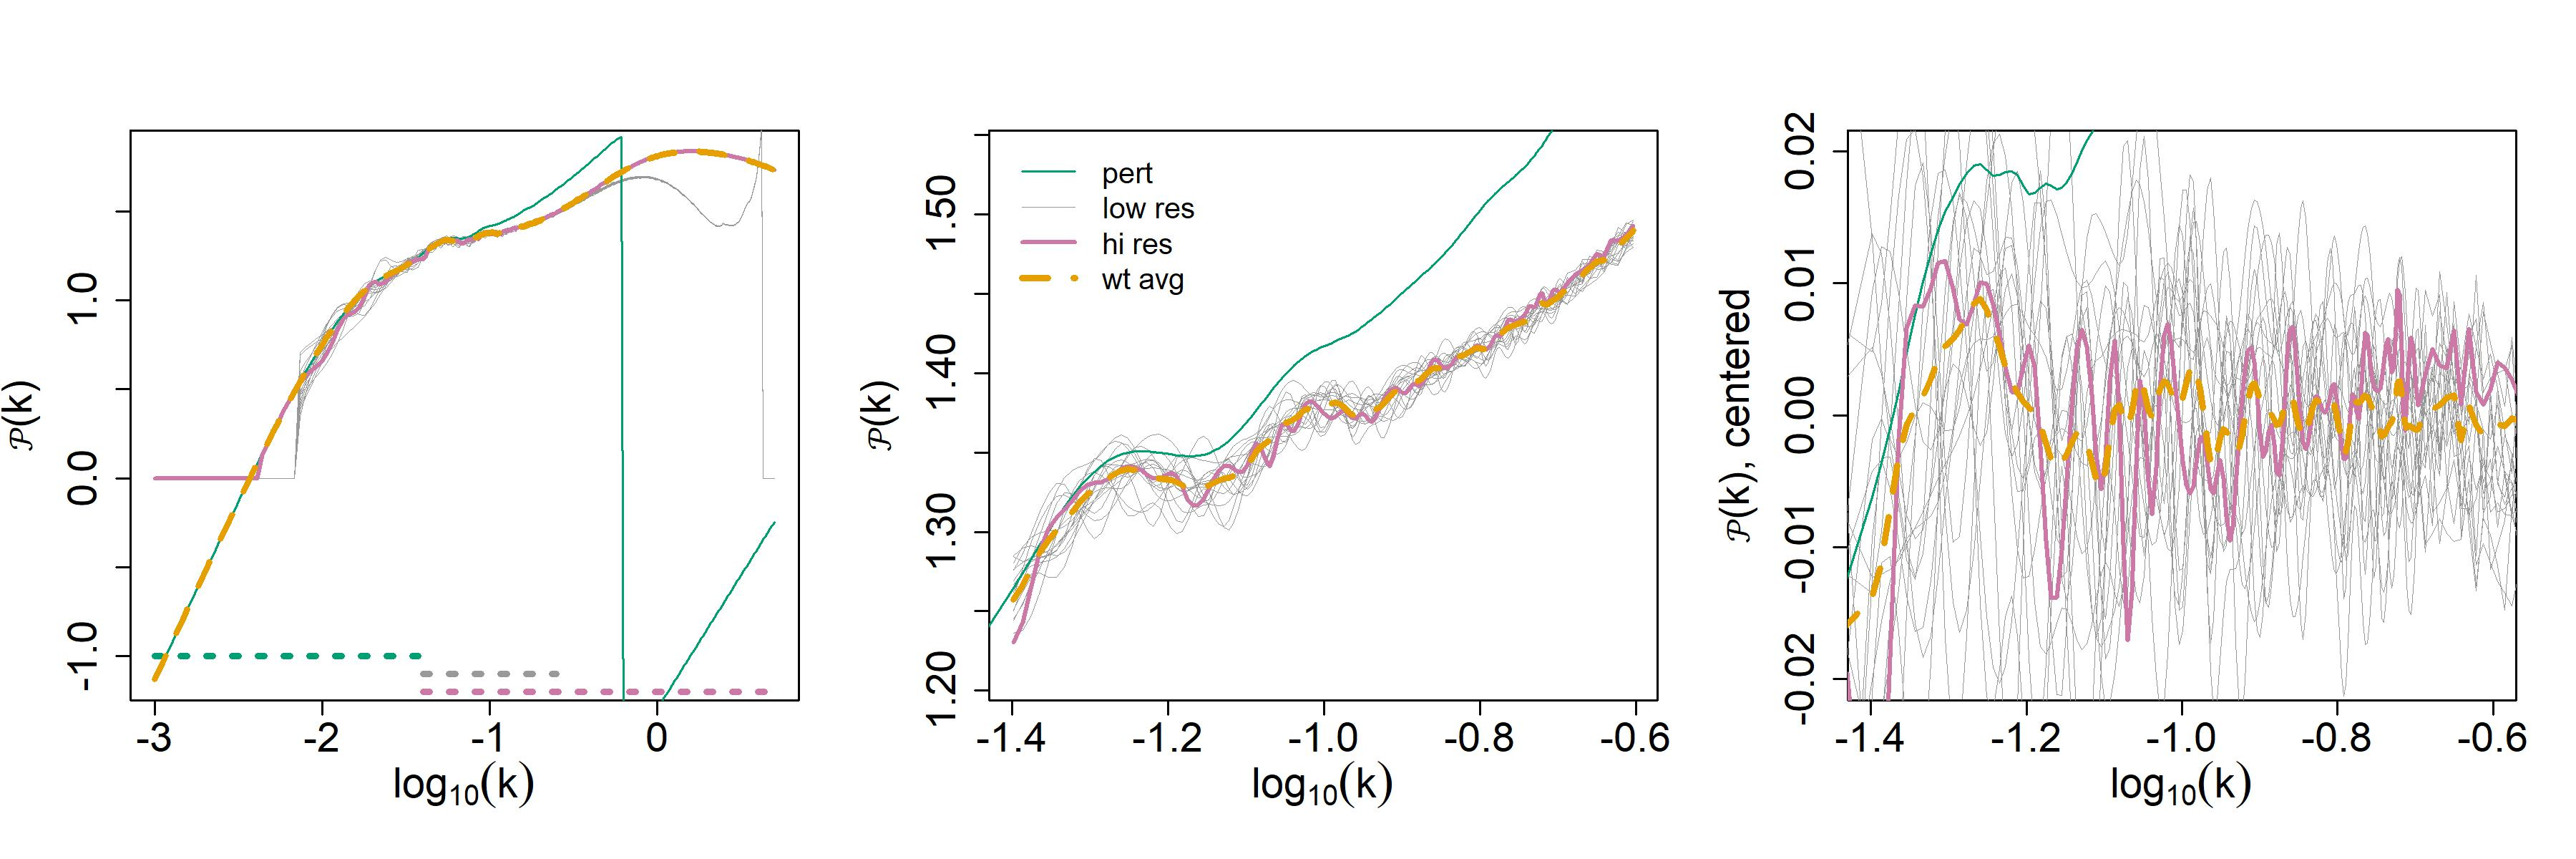
\includegraphics[width=\linewidth]{plot_data.jpeg}
    \caption{{\it Left:} The perturbation theory (solid green), low resolution runs (solid grey), 
    and high resolution run  (solid pink) for a particular cosmology. 
    The weighted average of these is shown in dashed orange. Dotted lines at the bottom
    indicate where each data type is deemed approximately unbiased. 
    {\it Middle:} Same as left, but restricted to wavenumber ($k$) values where the low resolution 
    runs are approximately unbiased.
    {\it Right:} Same as middle, but with LOESS-smooth weighted average subtracted.}
    \label{fig:plot_data}
\end{figure}

For each cosmology, Mira-Titan contains a batch of 18 simulated spectra: an inexpensive 
spectrum estimated from linear perturbation theory ($y_p$), 16 spectra estimated from 
low resolution simulations ($y_{\ell_r}, r \in \{1,\dots,16\}$), and one spectrum from 
a high resolution simulation ($y_h$). 
These spectra are represented as a function of wavenumber $k$.  Following 
\cite{moran2023mira}, we model on the emulation space 
$\mathcal{P}(k)=\log_{10}\left(\frac{k^{1.5}P(k)}{2\pi^2}\right)$, where $P(k)$ represents the
original spectra. Output is available for $n=351$ values of $k$, spanning
$0.001 \leq k \leq 5$, but each data type has unique wavenumber ranges
where it is deemed approximately unbiased. For $k<0.04$, only $y_p$ provides a reliable 
estimate of the true spectra. $y_{\ell_r}$ are valid for $0.04 \leq k \leq 0.25$, and 
$y_h$ is valid for $0.04 \leq k \leq 5$.  Figure \ref{fig:plot_data} shows an example 
of the output for a particular cosmology. When we focus on $k$ values where $y_{\ell_r}$ 
is valid (center panel), the spatially correlated errors of the low-resolution and high-resolution runs 
becomes apparent.

Notice, in the center/right panels of Figure \ref{fig:plot_data}, the precision of each
low/high resolution spectra increases as $k$ increases.  The curves get progressively 
tighter from left to right.  We would like to conveniently wrap this domain-specific 
knowledge inside our Bayesian framework later.  To this end, \cite{moran2023mira} 
used the multiple low- and high-resolution spectra across all cosmologies to
obtain precision estimates, $p_1,\dots, p_n$, across the $n$ 
wavenumber values using a log-log regression model. A multiplier $c\approx 3.73$ for 
the increase in precision from the low- to high- resolution output is also 
estimated with this regression model. 
We use these estimates to define three 
diagonal precision matrices, one for each data type (perturbation theory, 
low resolution average, and high resolution). Specifically, denote $\Lambda_p$, 
$\Lambda_\ell$, and $\Lambda_h$ as the $n\times n$ diagonal matrices with elements
\begin{equation}\label{eq:lambda}
\Lambda_p^{(ii)} = \begin{cases}
    10^8 &\text{for } k_i < 0.04 \\
    0  &\text{otherwise}\\
    \end{cases}
\quad
\Lambda_\ell^{(ii)} = \begin{cases}
    16p_i &\text{for } 0.04 \leq k_i < 0.25 \\
    0  &\text{otherwise}\\
    \end{cases}
\quad
\Lambda_h^{(ii)} = \begin{cases}
    cp_i &\text{for } 0.04 \leq k_i < 5 \\
    0  &\text{otherwise}\\
    \end{cases}
\end{equation}
for $i=1,\dots, n$.  In $\Lambda_p$, we use the sufficiently high precision 
of $10^8$ to impose the deterministic nature of the perturbation theory output.
In $\Lambda_\ell$, the multiplication by 16 accounts for the sample size of the
low resolution runs.
We then calculate a weighted average for each cosmology: 
$\bar y = \Lambda^{-1}(\Lambda_p y_p + \Lambda_{\ell} \bar{y}_\ell + \Lambda_h y_h)$, 
where $\Lambda = \Lambda_p + \Lambda_\ell + \Lambda_h$ and 
$\bar{y}_\ell = \frac{1}{16}\sum_{r=1}^{16} y_{\ell_r}$. In Figure \ref{fig:plot_data},
the weighted average is shown in dashed orange.  As an estimate of the true
underlying spectrum, the weighted average fluctuates too drastically.  
This is especially apparent after subtracting a LOESS-smoothed weighted average (right panel).
Although the weighted average incorporates all available observatons and 
expert knowledge regarding the precisions, it fails to account for the spatial 
dependence inherent in the smooth but stochastic spectra, which is pivotal to 
effectively inferring the true spectrum.

%We consider a training-testing split with 111 cosmologies used for estimation and 6 
%cosmologies held out for testing.  Our ultimate objective is to effectively predict
%the underlying power matter spectra for the held-out cosmologies based on their 
%8-dimensional input configuration (Section \ref{sec:pred}).  But first, we must 
%obtain effective estimates of the underlying spectrum for each training 
%cosmology (Section \ref{sec:hm_fit}). \textcolor{red}{(@Steve - maybe this is a
%good place to introduce the ``hold out'' and ``within sample'' terms?)}

\section{Bayesian Hierarchical Modeling for Particular Cosmologies}
\label{sec:hm_fit}

Here we describe our first contribution: the use of a Bayesian hierarchical model 
to estimate the underlying spectrum and quantify uncertainty for a particular cosmology.
Let input $X$ represent the vector with elements $x_i = \log_{10}(k_i)$ for $i=1,\dots,n$.
In the previous section, we used lowercase $\bar{y}$ to denote 
the observed weighted average; now, we use $\bar{Y}$ to indicate the corresponding 
random variable within the statistical model.  
%Together, $X$ and $\bar{Y}$ comprise the 
%training data for a particular cosmology. 
$\bar{Y}$ is typically pre-processed
based on domain expertise.  Pre-processing for Mira-Titan was described in Section 
\ref{sec:data}; we will detail pre-processing 
for the CAMB suite in Section \ref{subsec:camb}.

\subsection{Model Specification}
\label{sec:mod_spec}

Let $S$ represent the true (but unknown) underlying power matter spectrum for
a particular cosmology.  We consider $\bar{Y}$ a noisy realization of $S$.
Specifically, we assume $\bar{Y}$ is a random realization of a Gaussian 
process centered at $S$ with some covariance, i.e., 
$\bar{Y}\mid S \sim \mathrm{GP}(S, \Sigma_\varepsilon)$.  While previous works
have considered diagonal $\Sigma_\varepsilon$ \citep{moran2023mira}, we find it
essential to account for the smoothly varying spatial dependence
(as visualized in Figure \ref{fig:plot_data}).  We thus specify a dense 
covariance matrix $\Sigma_\varepsilon$ that simulataneously
allows us to model the correlated errors and build domain-matter expertise
into the prior. To this end, we embrace variations of the Mat\'ern kernel 
\citep{stein1999interpolation}, tailored to each cosmology (more on this in later 
subsections). 

We next place a Gaussian process prior on $S$, i.e.,
$S\sim \mathrm{GP}\left(\boldsymbol{\mu}_S, \Sigma_S(\cdot)\right)$, again with a 
Mat\'ern kernel. Here, we set $\boldsymbol{\mu}_S=\mathbf{0}$, although our model
is applicable to any selection of $\boldsymbol{\mu}_S$. Standard practice would 
use locations $X$ as the inputs to kernel $\Sigma_S(\cdot)$, yet we have found that 
prior to lack sufficient flexibility for our motivating
application.  In the Mira-Titan setting, some nonstationarity is expected due to 
baryonic acoustic oscillations when $-2 \leq \log_{10}(k) \leq -1$. To account 
for this, we incorporate a latent monotonic Gaussian process \citep[monoGP;][]{barnett2025monotonic},
which accommodates nonstationarity by warping $X$ via 
$W \sim \mathrm{monoGP}\left(\boldsymbol{\mu}_W, \Sigma_W(X)\right)$.
$W$ is also an $n$-vector whose entries $w_i$ correspond to warped versions of each $x_i$.
Again, we set $\boldsymbol{\mu}_W = \mathbf{0}$ without loss of generality (we have
found $\boldsymbol{\mu}_W = X$ works similarly).
Ultimately, this yields the following hierarchical model:
\begin{equation}\label{eq:dgphm}
\begin{aligned}
\bar{Y}\mid S,\Sigma_\varepsilon &\sim \mathrm{GP}(S,\Sigma_\varepsilon) \\
S\mid W &\sim \mathrm{GP}\left(\mathbf{0}, \Sigma_S(W)\right) \\
W &\sim \mathrm{monoGP}\left(\mathbf{0}, \Sigma_W(X)\right).
\end{aligned}
\end{equation}
The functional composition of GPs in the latter two lines forms a ``deep Gaussian process'' 
\citep{damianou2013deep,dunlop2018deep}. Additional latent layers could be considered, 
although we find one is sufficient.

For both $\Sigma_S$ and $\Sigma_W$, we use Mat\`ern kernels with smoothness of $2.5$,
unit scale, and unique lengthscales:
\begin{equation}\label{eq:cov}
\begin{array}{l}
\Sigma_S(W)^{i,j} = K\left(||w_i - w_j||^2, \theta_S\right) \\[7pt]
\Sigma_W(X)^{i,j} = K\left(||x_i - x_j||^2, \theta_W\right)
\end{array}
\quad\textrm{where}\quad
K(d, \theta) = \left( 1 + \frac{\sqrt{5}d}{\sqrt{\theta}} + 
  \frac{5d^2}{3\theta}\right) \exp\left(-\frac{\sqrt{5}d}{\sqrt{\theta}}\right).
\end{equation}
In our one-dimensional setting, we embrace unit scale on $S$ to preserve parsimony 
and identifiability with $\theta_S$ \citep{zhang2004inconsistent}.
Unit scale on latent $W$ was recommended by \citet{sauer2023active} for similar reasons.

\subsection{Bayesian Inference}\label{sec:inference}

Our inferential goal is to obtain the posterior distribution of 
$S\mid\bar{Y},\Sigma_\varepsilon$, but this requires inferring latent $W$.  
We first integrate over $S$ to condense our hierarchical model of Eq.~(\ref{eq:dgphm}) into
\begin{align}
\label{eq:likelihood}
\bar{Y} \mid W, \Sigma_\varepsilon &\sim \textrm{GP}(\mathbf{0}, \Sigma_S(W) + \Sigma_\varepsilon) \\
\label{eq:prior}
W &\sim \mathrm{monoGP}\left(\mathbf{0}, \Sigma_W(X)\right)
\end{align}
A detailed derivation, including generalizations for 
$\boldsymbol{\mu}_S\neq\mathbf{0}$, is provided in \ref{sec:apdx_int_lik}. 
The incorporation of $\Sigma_\epsilon$ in the
Gaussian likelihood of this outer layer is an essential upgrade to previous DGP inferential schemes.
This covariance incorporates knowledge of the smoothly varying dynamics from which $\bar{Y}$ was
generated.

We embrace fully-Bayesian inference of latent $W$ and kernel hyperparameters $\{\theta_S, \theta_W\}$.
Specifically, we use elliptical slice sampling \citep[ESS;][]{murray2010elliptical} to 
generate posterior samples of $W$, using Eq.~(\ref{eq:prior}) for proposal generation and 
Eq.~(\ref{eq:likelihood}) for likelihood-based acceptance.  
For $\theta_S$ and $\theta_W$, after pre-scaling, we adopt the default prior specifications 
provided in the {\tt deepgp} {\sf R}-package \citep{deepgp}.
We then integrate Metropolis-Hastings sampling of these parameters in a Gibbs framework 
with the ESS sampling of $W$ \citep{sauer2023active}.

Given burned-in posterior samples $W^{(t)}$ and $\theta_S^{(t)}$
for $t\in\mathcal{T}$ ($\theta_W^{(t)}$ is only used to sample $W^{(t)}$), 
we may leverage Bayes' Theorem to obtain the
posterior distribution of the true power matter spectrum for a particular cosmology as
\[
S^{(t)}\mid\bar{Y}, \Sigma_\varepsilon \sim \mathrm{GP}(m^{(t)}, C^{(t)})
\quad\textrm{where}\quad
\begin{array}{rl}
C^{(t)}&=\left(\Sigma_S(W^{(t)})^{-1}+\Sigma_\varepsilon^{-1}\right)^{-1} \\
m^{(t)}&=C^{(t)}\left(\Sigma_\varepsilon^{-1}\bar{Y}\right).
% "+\Sigma_S(W^{(t)})^{-1}\boldsymbol{\mu}" removed from m^t when mu=0
\end{array}
\] 
This form is simplified for $\boldsymbol{\mu}_S=\mathbf{0}$; a general derivation 
is provided in \ref{sec:apdx_SgivenY}.  This closed-form enables direct posterior
sampling of $S^{(t)}$ at discrete locations $x_i$ for $i=1,\dots, n$.  
We draw samples accordingly and compute their average 
to obtain our posterior mean for a particular cosmology. 
Additionally, we quantify uncertainty by finding the 2.5th and 97.5th percentiles 
of the posterior draws at each index to obtain a 95\% credible interval.
We denote our inference procedure for the hierarchical model of Eq.~(\ref{eq:dgphm}) as
``DGP.FCO'' given its deep Gaussian process foundation with additional hierarchical
structure to incorporate functional correlated outputs (FCO).

\subsection{Simulation Study}
\label{subsec:sim}

We compare DGP.FCO to competing models with a simulation study where the underlying 
true curve is known. Following \cite{moran2023mira}, we consider two test functions 
defined as
\[
\begin{aligned}
  f_1(x) &= m_1 \exp\left(-\frac{u_1x}{2}\right) * 
  \cos\left(x\sqrt{25-\left(\frac{u_1}{2}\right)^2}\right) - \frac{m_1x}{5}\\
  f_2(x) &= \exp\left(-m_2(x-3)^2\right) + 
  \exp\left(-u_2(x-1)^2\right)-0.05\sin\left(8(x-1.9)\right).
\end{aligned}
\]
For additional variation, the values of $m_1, m_2, u_1,$ and $u_2$ are randomly selected from
$m_1 \sim \text{Uniform}(0.5,1.5)$, $u_1 \sim \text{Uniform}(1.5,2.5)$, and $m_2,u_2 
\sim \text{Uniform}(0.6,1.4)$. The outputs of $f_1$ and $f_2$ (conditional on $m_1/u_1$ and 
$m_2,u_2$), determine the true function values for each simulation.
      
For each of the two true functions, we consider two variance settings $A$ and $B$, where 
matrices $\Sigma_A$ and $\Sigma_B$ have a Mat\'ern kernel with smoothness of 2.5,
as defined in Eq.~(\ref{eq:cov}). 
We obtain function realizations at $x=\{0, 0.1, \dots, 
3.9, 4.0\}$, so that each function draw contains $n=41$ observations. We draw $r$-many 
realizations from a GP with mean $f_1$ or $f_2$ and spatially varying covariance
$\Sigma_A$ or $\Sigma_B$, where:  

\[
\begin{aligned}
\Sigma_A &= 0.0225 * K(||x_i - x_j||^2, 0.01), \\
\Sigma_B &= s^\top Ms \quad\textrm{where}\quad M = 0.1 * K(||x_i - x_j||^2, 0.05)
\quad\textrm{and}\quad s = 1.5^{-x/2}.
\end{aligned}
\]
Observations are kept noise-free, but we do add a jitter of $10^{-8}$ to the diagonal of $\Sigma_A$ 
and $\Sigma_B$ for numerical stability.  Within $\Sigma_B$, $s$ introduces a degree of
nonstationarity, more effectively mimicing the behavior of the 
CAMB and Mira-Titan datasets.  Examples of simulation output are showin in 
Figure \ref{fig:run_sim_f1A_f2B}.

\begin{figure}
    \centering
    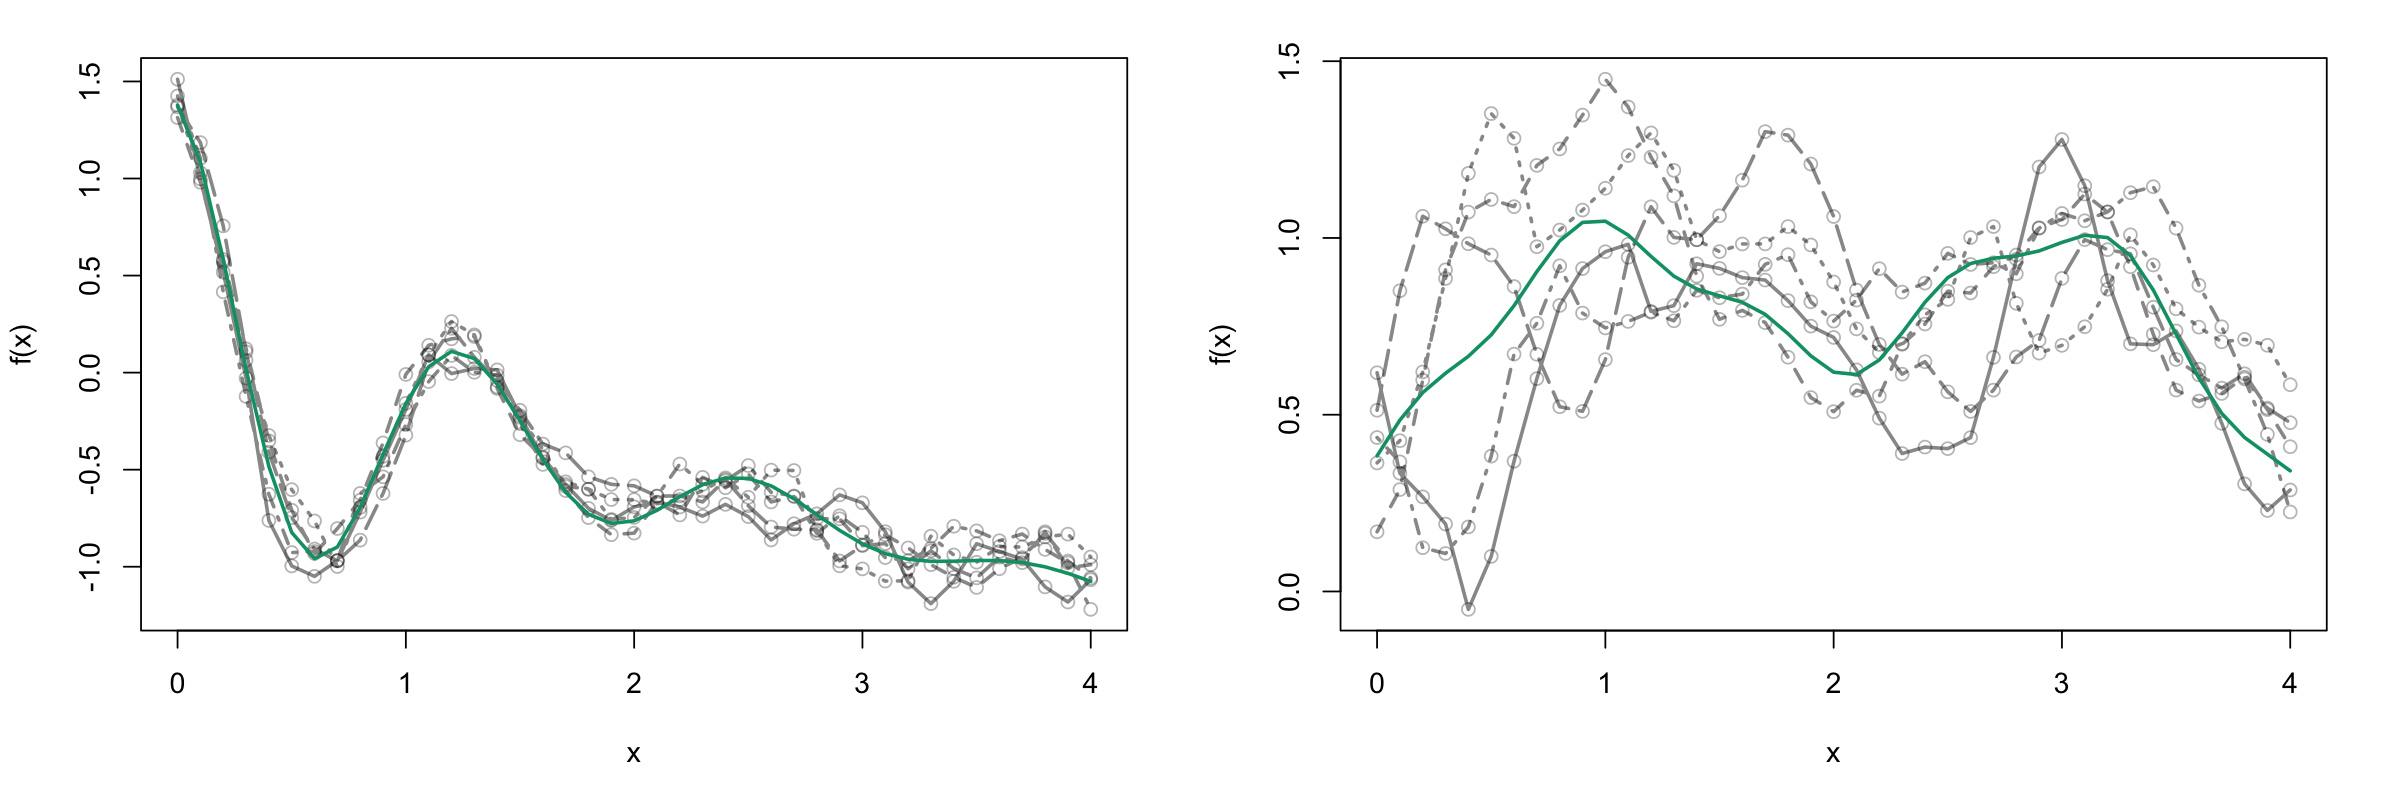
\includegraphics[width=\textwidth]{run_sim_f1A_f2B.png}
    \caption{Illustration of simulation output, each with $r=5$ function realizations. The true function
             is shown in solid green, while the gray lines and points indicate the realizations. 
             {\it Left:} $f_1$ with variance setting $A$. 
             {\it Right:} $f_2$ with variance setting $B$.}   
    \label{fig:run_sim_f1A_f2B}
\end{figure}

\begin{figure}[t]
    \centering
    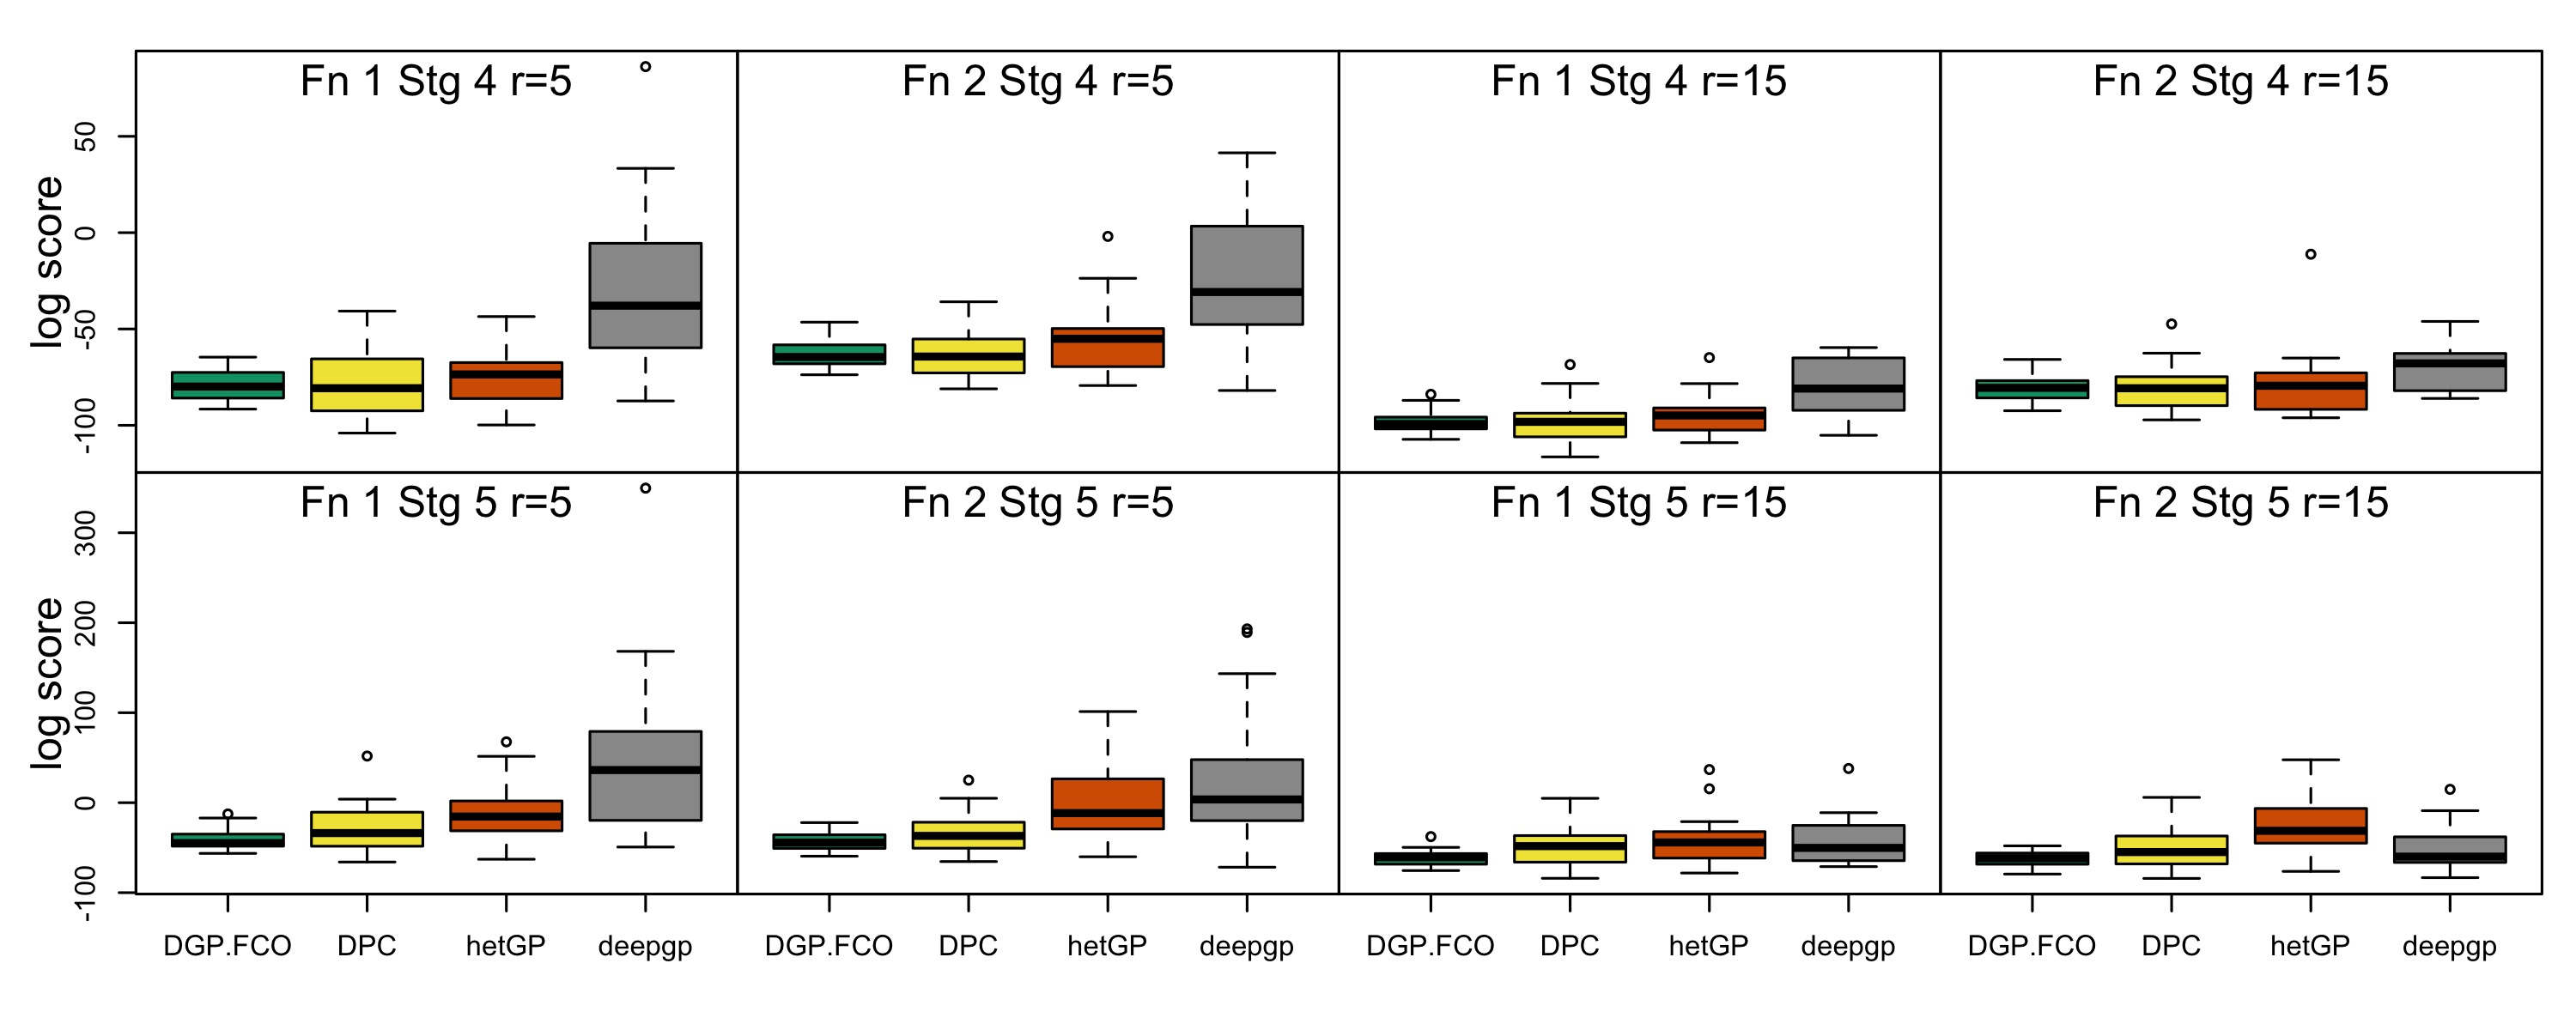
\includegraphics[width=\textwidth]{sims_logS.jpeg}
    \caption{Boxplot of log scores (20 repetitions, lower is better) for each 
             simulated scenario.  Each column represents a function/covariance 
             pair, and each row shows results for $r=5$ (top) or $r=15$ (bottom).}
    \label{fig:sims_logS}
\end{figure}

For each simulated function and variance specification, we conduct 20 Monte Carlo repetitions
with re-randomized $m_1, u_1, m_2, u_2$.  We consider $r = 5$ and $r = 15$.
We compare to an out-of-the-box DGP from the 
\texttt{deepgp} package \citep{sauer2023active}, a heteroskedastic GP from
the \texttt{hetGP} package \citep{binois2018practical, binois2021hetgp}, and
a deep process convolution (DPC) approach, which is utilized within Cosmic 
Emu \citep{moran2023mira}.  These competing methods view the training data as 
noisy observations with no spatial dependence (i.e., they view the gray dots of
Figure \ref{fig:run_sim_f1A_f2B} without the lines). In
contrast, our method leverages the fact that the observations represent $r$-many
smooth functional realizations in order to estimate parameters
within $\Sigma_\epsilon$ that account for the spatial dependence.
Our method achieves this by first pre-scaling the functional realizations by the
precision values (to account for nonstationarity), and then using maximum likelihood
estimation to obtain estimates of the marginal variance and lengthscale of the 
Mat\'ern spatial correlation function. We use these estimates and the precision 
information to construct $\Sigma_\varepsilon$.

We evaluate performance of each method using log score, a proper scoring 
rule which takes both accuracy and UQ into 
consideration \citep[][lower is better]{gneiting2007strictly}.
Results are shown in Figure \ref{fig:sims_logS}.  Our DGP.FCO 
model performs favorably across the board; accounting for the spatial 
dependence between the observations results in more effective UQ.
We relegate mean squared error (MSE) results to \ref{sec:apdx_sims}, because
MSE neglects UQ and was comparable across competing methods.

\subsection{CAMB Estimation}
\label{subsec:camb}

The CAMB \citep{lewis2011CAMB} dataset contains power spectra based
on six cosmological parameter settings. It includes sixty-four cosmologies,
each containing fifteen low-resolution spectra ($y_{l_r}$) and one high-resolution spectrum ($y_h$).
Each spectrum is observed along the same grid of wavenumbers ($k_i$ for $i=1,\dots,n$). 
Unlike the Mira-Titan suite, this dataset includes an infinite-resolution 
spectrum ($y_c)$ which can be treated as the true spectrum for each cosmology,
allowing us to assess model performance. An illustration of the first cosmology 
from CAMB is shown in Figure \ref{fig:fit_camb}.  The ``true'' infinite-resolution 
spectrum is notably smoother than its low- and high-resolution counterparts.

\begin{figure}
    \centering
    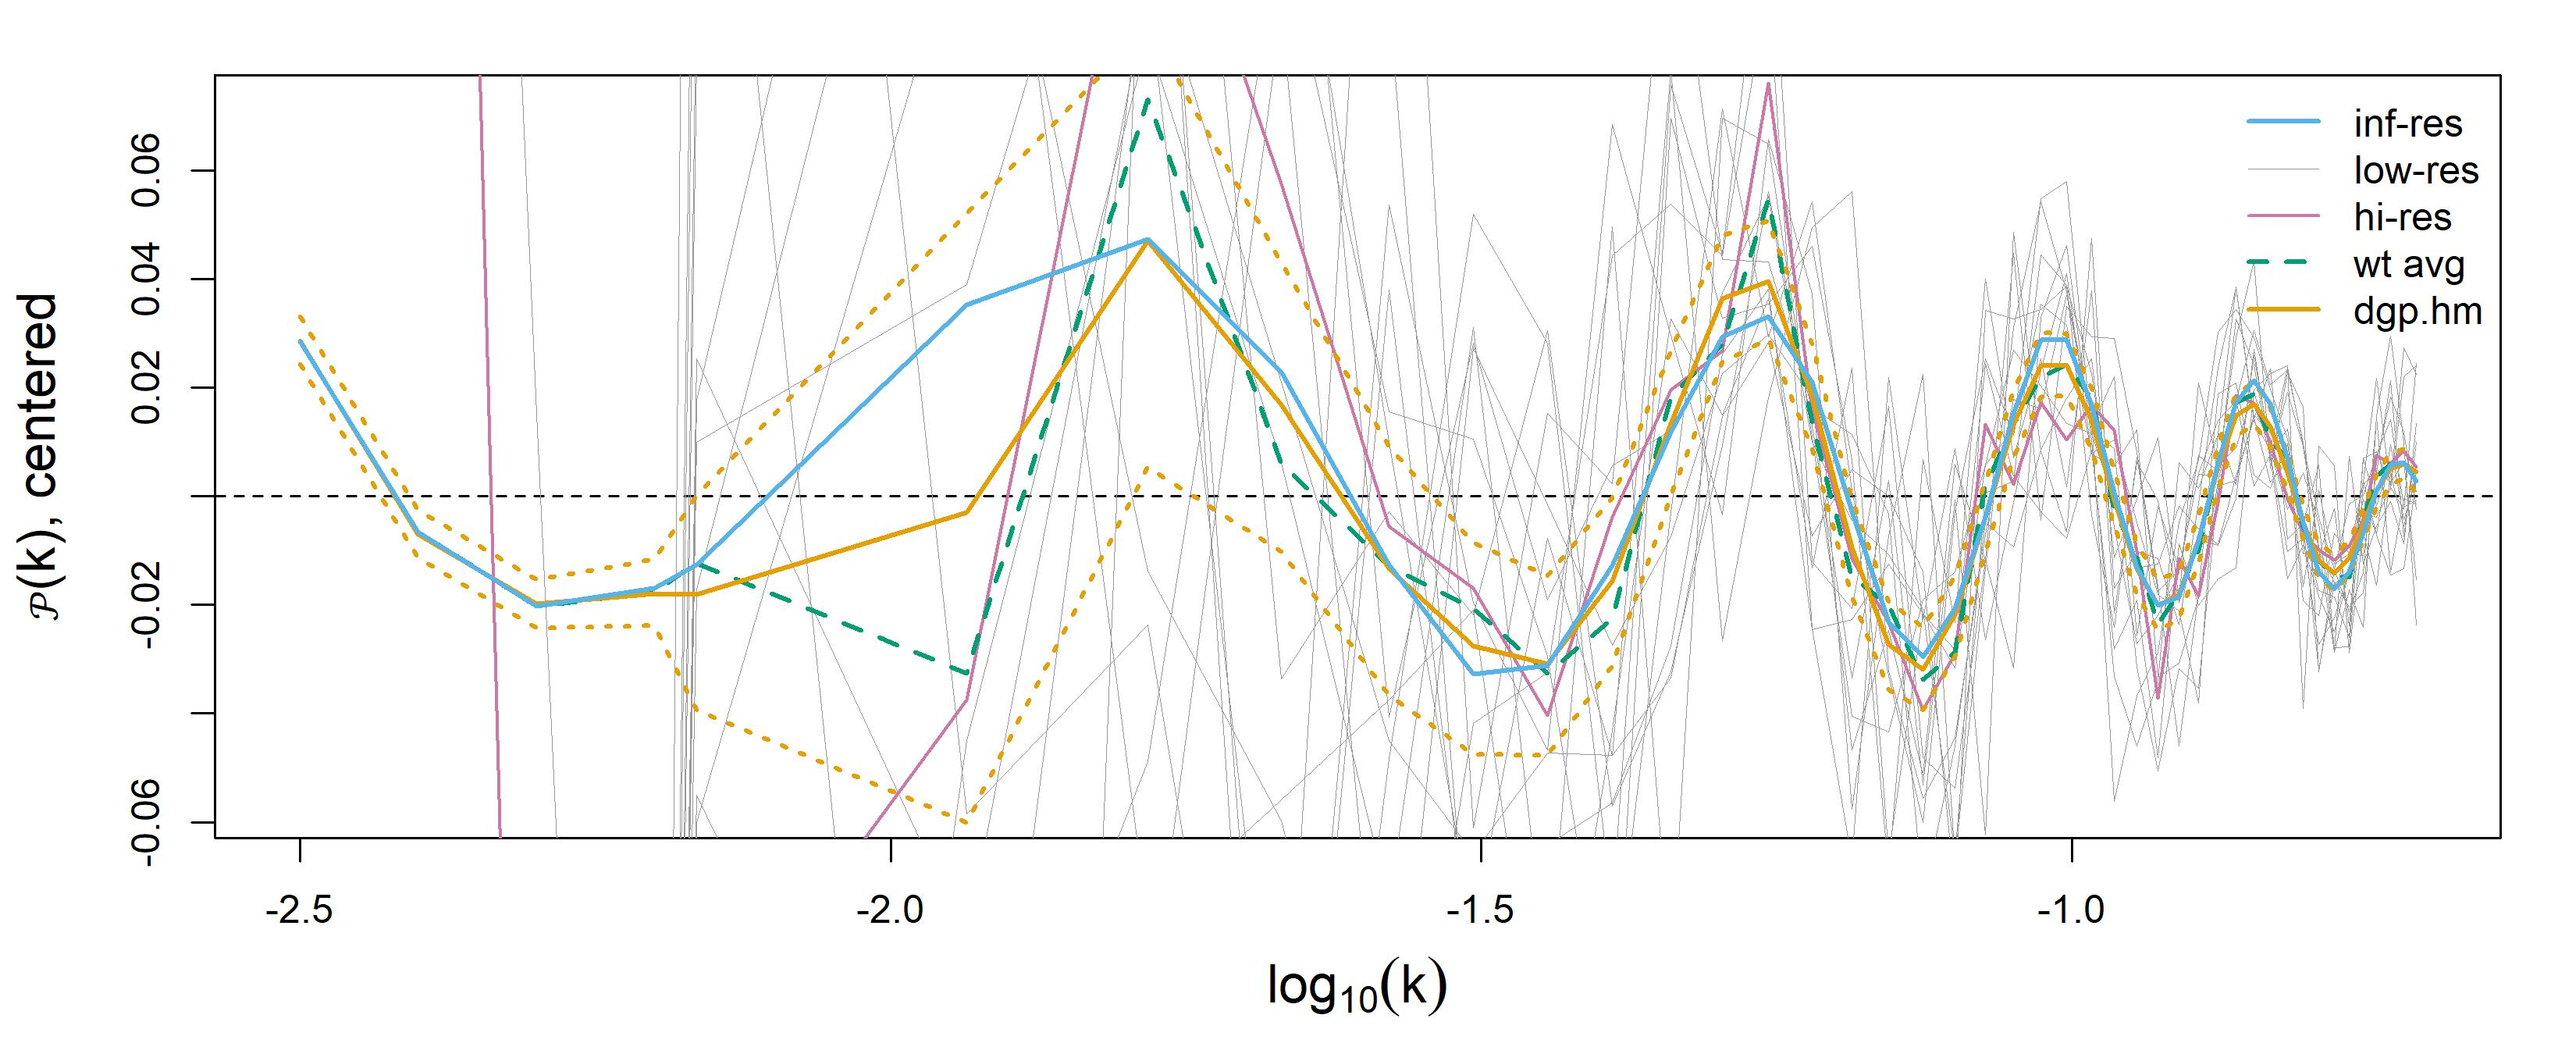
\includegraphics[width=\textwidth]{CAMB_fit_model1.jpeg}
    \caption{Example of DGP.FCO model fit for the first batch of model runs from the CAMB data, 
             with a LOESS mean of the weighted average subtracted to emphasize details. We can 
             compare the orange lines (posterior mean and dotted 95\% credible interval) to the 
             light blue line, representing the infinite-resolution ``true" spectrum.}   
    \label{fig:fit_camb}
\end{figure}

To imitate the role of the perturbation theory output of Mira-Titan, we anchor 
estimates of the CAMB power spectrum at the infinite-resolution for 
$\log_{10}(k) < -2.2$, and then rely strictly on the low- and high-resolution 
runs for $k$ above this (note the transition
in Figure \ref{fig:fit_camb} at $\log_{10}(k) = -2.2$). To compute $\bar{y}$ and $\Sigma_\epsilon$,
we first use a log-log regression model to obtain precision estimates $\Lambda_\ell$ and $\Lambda_h$
for the low- and high-resolution runs respectively, as outlined in Section \ref{sec:data}. 
To anchor estimates at low resolutions, we define the diagonal matrix $\Lambda_c$ with 
$\Lambda_c^{(ii)}=10^8$ for $\log_{10}(k_i) < -2.2$ ($0$ otherwise).
We then compute the weighted average as: $\bar y = \Lambda^{-1}(\Lambda_c y_c + 
\Lambda_{\ell} \bar{y}_\ell + \Lambda_h y_h)$, where $\Lambda = \Lambda_c + \Lambda_\ell + \Lambda_h$ 
and $\bar{y}_\ell = \frac{1}{15}\sum_{r=1}^{15} y_{\ell_r}$.
For the CAMB data, spatial correlation decays very quickly
(compare the smoothly varying low-resolution runs of Mira-Titan in Figure \ref{fig:plot_data} 
with the jagged low-resolution runs of CAMB in Figure \ref{fig:fit_camb}). 
Although we considered a Mat\'ern kernel for $\Sigma_\epsilon$ here, we found the covariance
to decay so quickly ($\theta\approx 0$) that a diagonal covariance would suffice.
Therefore, we drop spatial dependence and specify $\Sigma_\varepsilon = 
(\Lambda_c+\Lambda_\ell+\Lambda_h)^{-1}$.  

We fit our DGP.FCO model to the low- and high-resolution runs of each CAMB cosmology for
later use in Section \ref{sec:pred}.  For now, we provide an illustration of the DGP.FCO
prediction (solid yellow) and credible intervals (dashed yellow) for a single 
CAMB cosmology in Figure \ref{fig:fit_camb}.  Our posterior mean provides an effective estimate
of the ``true'' infinite-resolution run.  It aptly smooths over the peaks where 
both the high-resolution run and the weighted average significantly deviate from the truth
($\log_{10}(k)\approx -1.8,-1.3$). Our model also provides effective UQ, appropriately shrinking
credible intervals as precision increases for larger $k$.

\subsection{Mira-Titan Estimation}
\label{subsec:mira_fit}

Here, we revisit the Mira-Titan suite described in Section \ref{sec:data} to provide
final details for our estimation of the true (but unknown) matter power spectrum for
each cosmology.  Recall, with $\Lambda_p$, $\Lambda_\ell$, and $\Lambda_h$ as 
defined in Eq.~(\ref{eq:lambda}), we compute
$\bar y = \Lambda^{-1}(\Lambda_p y_p + \Lambda_{\ell} \bar{y}_\ell + \Lambda_h y_h)$, 
where $\Lambda = \Lambda_p + \Lambda_\ell + \Lambda_h$.
Turning to $\Sigma_\epsilon$, since the low-resolution spectra 
vary smoothly about $S$ (e.g., Figure \ref{fig:plot_data}), we prefer a dense 
covariance ($\Sigma_\ell$) for wavelengths $0.04 \leq k < 0.25$.
In previous work, we considered multiple candidates for 
$\Sigma_\varepsilon$ \citep{walsh2023bayesian} and found that a Mat\'ern covariance 
for $\Sigma_\ell$ trained on the low-resolution runs (pre-scaled by the precision 
values and subtracting a LOESS-smoothed average) performs the best. 
We specify this structure within $\Sigma_\varepsilon$ and refer readers 
to \cite{walsh2023bayesian} for a more detailed exposition. This yields 
$\Sigma_\varepsilon=\left(\Lambda_p^{-1} + \Sigma_\ell + \Lambda_h^{-1}\right)^{-1}$.

We then fit our DGP.FCO model on each of 111 training cosmologies, reserving 6 cosmologies
for later hold-out testing.  Figure \ref{fig:plot_fit} 
visualizes the DGP.FCO fit for the first training cosmology.  We center the plot
by subtracting the posterior mean in order to more easily visualize the credible
interval bounds.  The UQ from the DGP.FCO model accounts for varying precisions 
across differing $k$ values, as well as the spatial correlation within the 
functional realizations.  To provide insight into the nonstationarity of the power
matter spectrum, the right panel of Figure \ref{fig:plot_fit} shows burned-in elliptical 
slice samples of $W$.
These warpings depart from the identiy mapping around $x\approx-1$, 
stretching inputs where dynamics are shifting more rapidly for larger $k$ values.

\begin{figure}[ht]
    \centering
    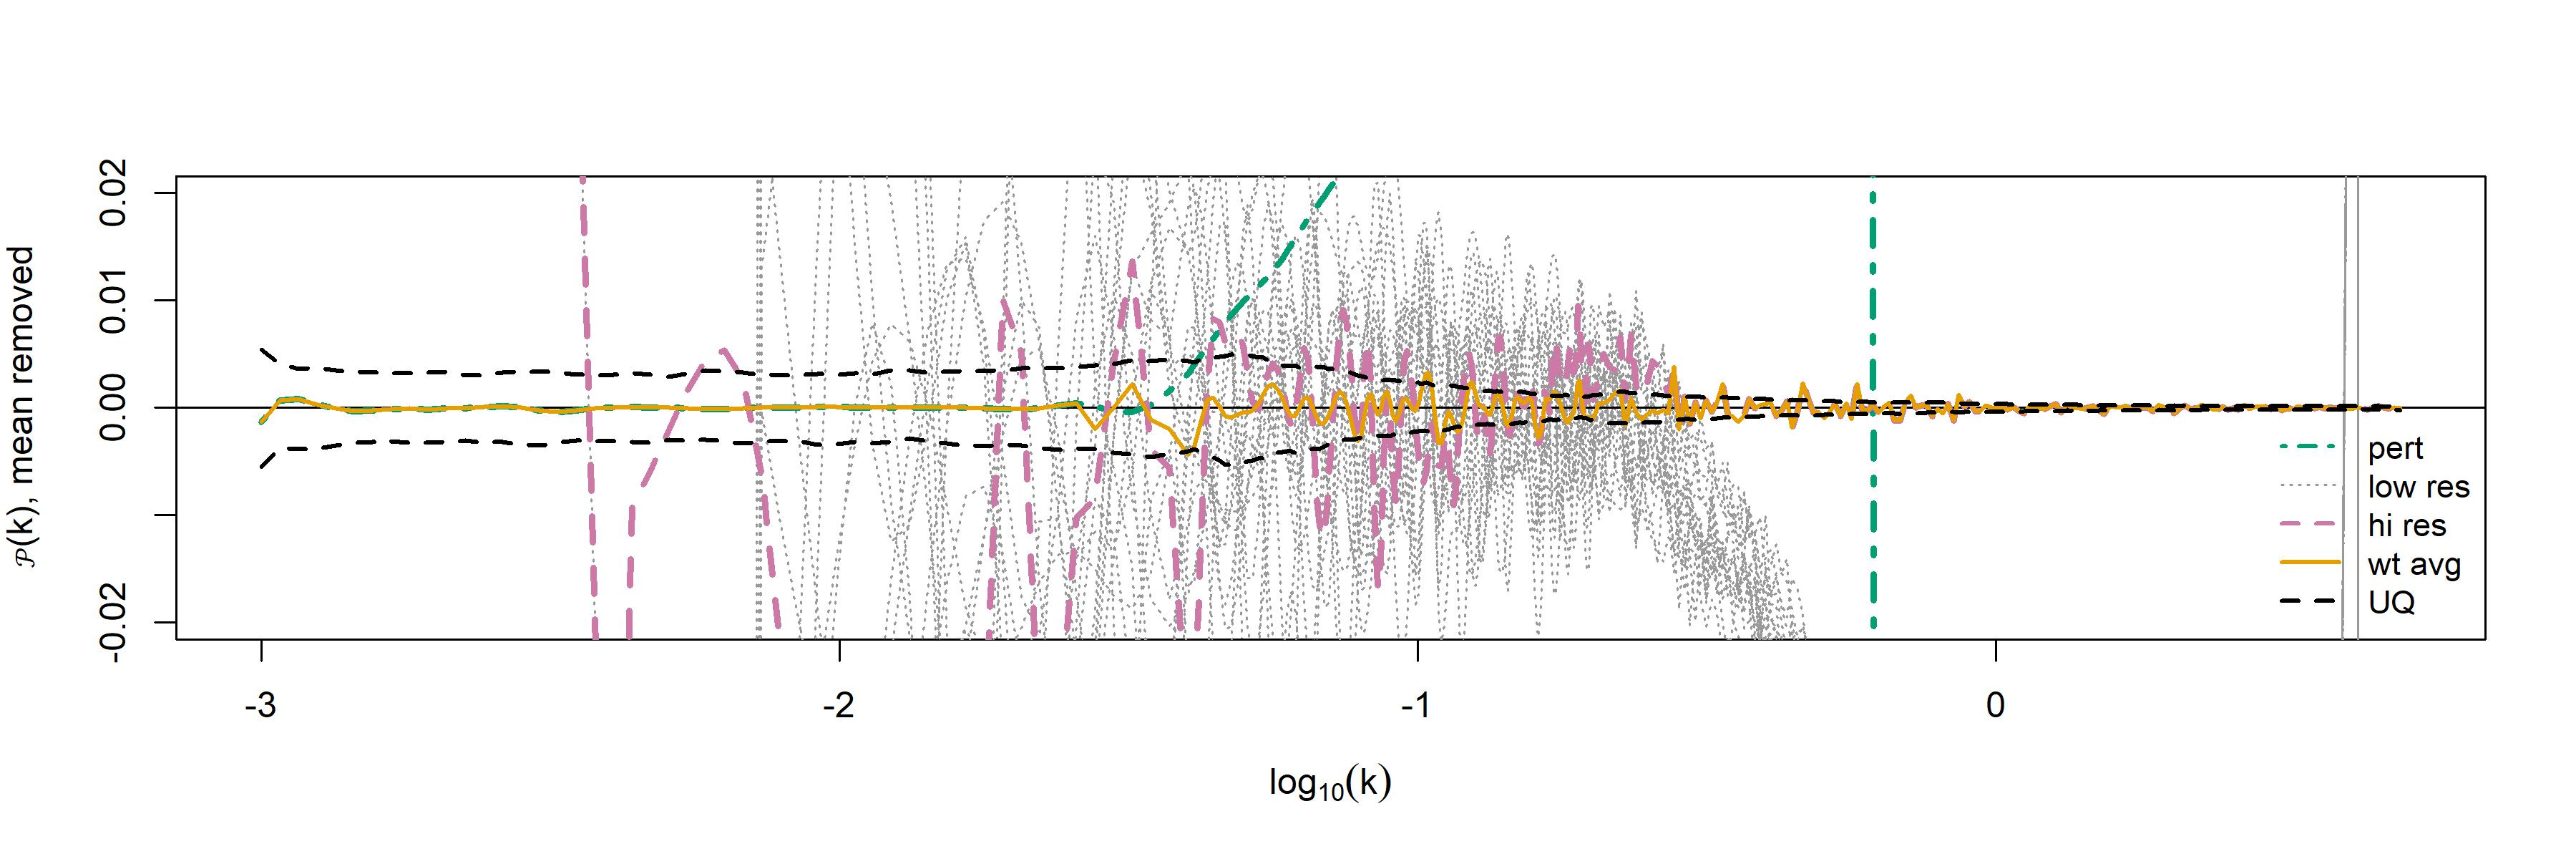
\includegraphics[width=6in]{plot_fit.jpeg}
    \caption{{\it Left:} 95\% credible intervals for the power spectrum of the first Mira-Titan
    cosmology (centered by the predicted posterior mean). Perturbation theory, 
    low-resolution, and high-resolution runs are shown for context. {\it Right:} Posterior draws
    of $W$, illustrating nonstationary behavior by departing from a linear (identity) mapping.}
    \label{fig:plot_fit}
\end{figure}

\section{Prediction for Unobserved Cosmologies}
\label{sec:pred}

Here we detail our second contribution - using the Bayesian DGP.FCO model predictions
from training cosmologies to predict the matter power spectra for held-out cosmologies. 
%This is achieved with modeling the weights of different basis functions as GPs.

\subsection{Functional Prediction Model}
\label{subsec:pca}

Let $\psi \in \mathbb{R}^{p_\psi}$ denote the set of parameters that define a particular cosmology.
Mira-Titan has 8 such parameters as described in Section \ref{sec:data}; CAMB has 6.
Our goal is to effectively predict the power matter spectrum as a function of $\psi$, i.e., $\hat{S}(\psi)$, 
for a held-out cosmology.  We observe $m$-many training cosmologies and fit our DGP.FCO 
model (Section \ref{sec:inference}) to each one.  Let $\hat{S}_j$ for $j \in \{1,\ldots,m\}$ denote
the estimated posterior mean of each training cosmology.  In total, our training data comprises
the $p_\psi$-dimensional input $\psi_j$ and the $n$-dimensional output $\hat{S}_j$ (which is a 
function of $x_i = \log_{10}(k_i)$) for $j \in \{1,\ldots,m\}$.

To handle the functional nature of this output, we reformulate the problem using principal
components \citep[PCs; e.g.,][]{banerjee2014linear}.  
We first center all $\hat{S}_j$ by subtracting $\bar{S} = \frac{1}{m}\sum_{j=1}^{m} \hat{S}_j$, 
then we combine them into an $n\times m$ matrix $\boldsymbol\eta$.  We use the first $p_\eta$ 
principal components to decompose $\boldsymbol\eta = B\Gamma^\top$ where $B$ is the 
$n\times p_\eta$ matrix of basis functions and $\Gamma$ is the $m\times p_\eta$ matrix of basis weights.  
Details on this decomposition are reserved for \ref{sec:apdx_basis}. For both the CAMB and Mira-Titan 
datasets, we set $p_\eta=10$. As a visual, the left panel of Figure \ref{fig:mean_PCs_oneW} shows 
$\bar{S}$ for the Mira-Titan training cosmologies.  The center panel shows the $p_\eta$ basis functions.

\begin{figure}
    \centering
    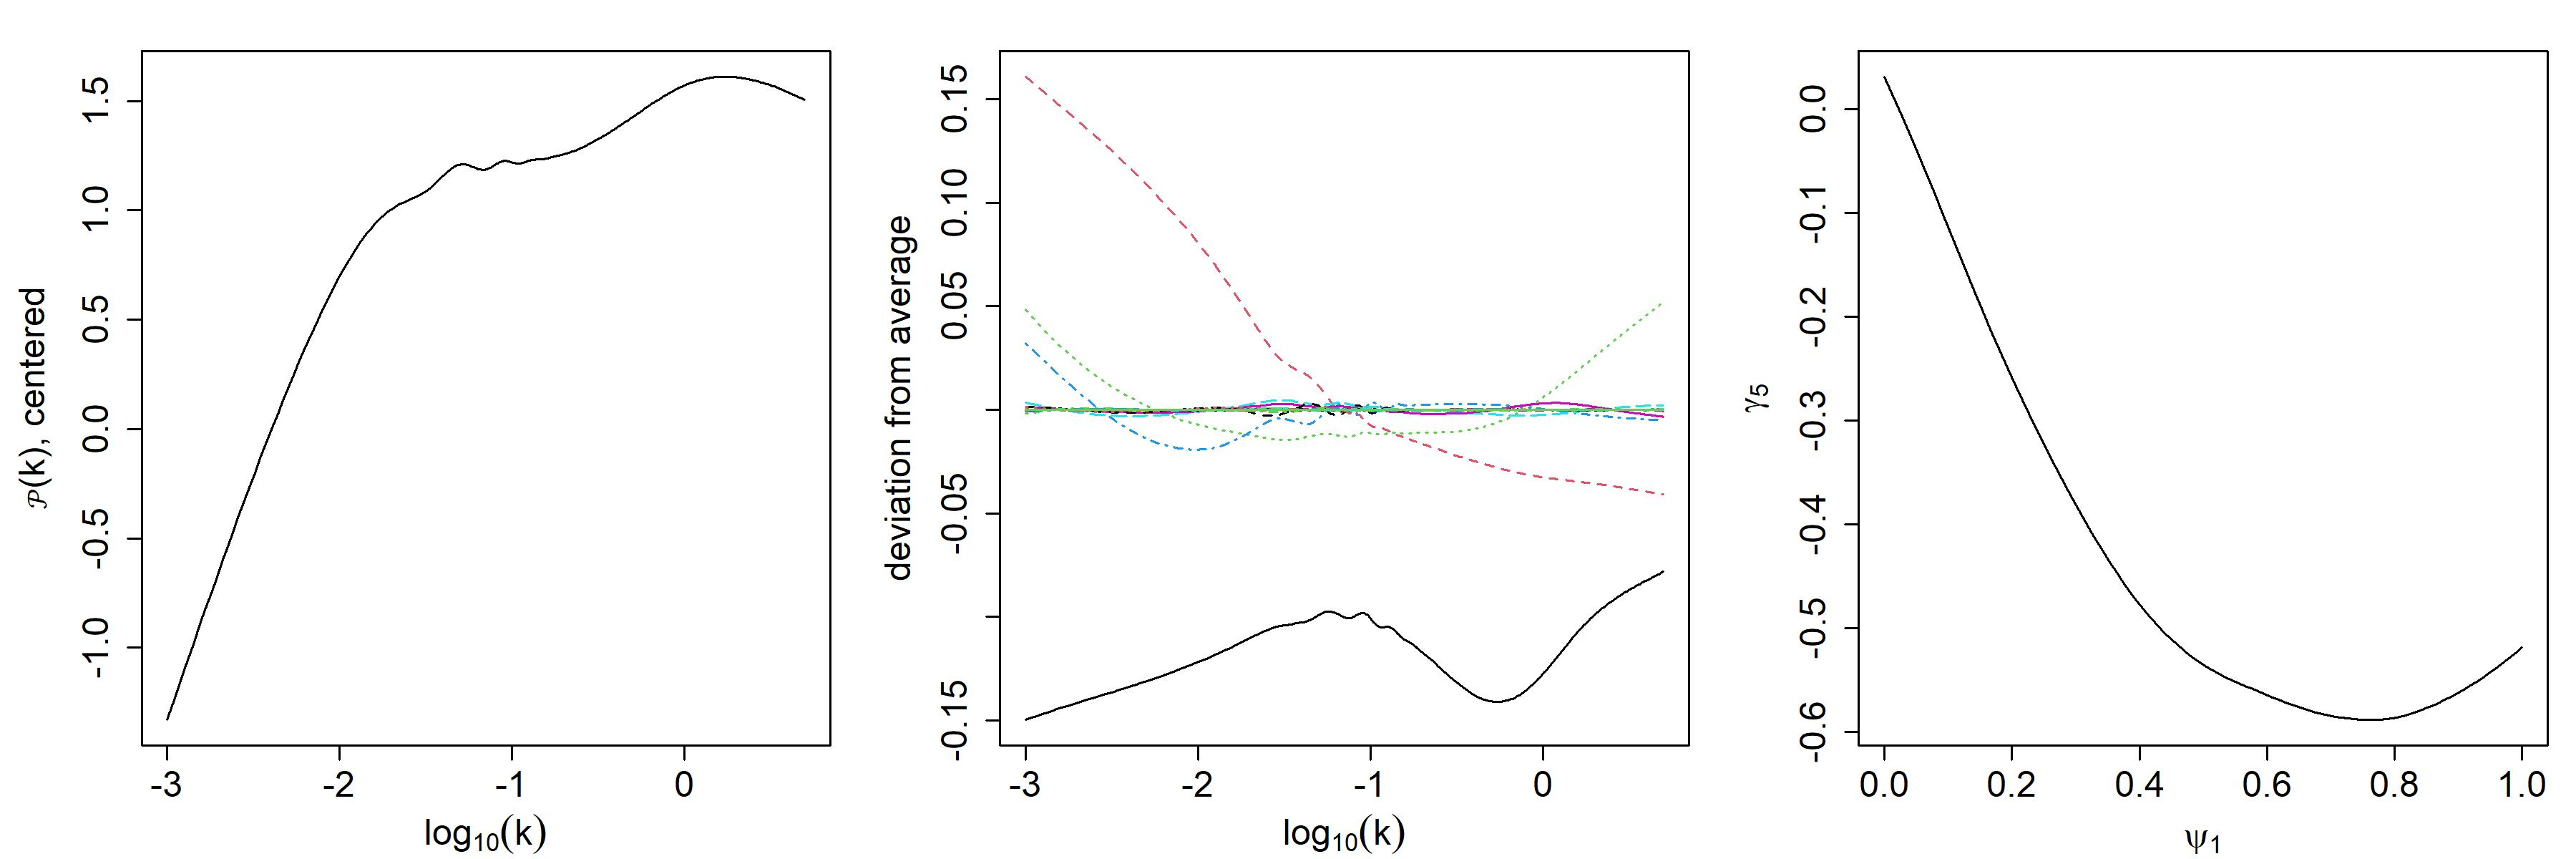
\includegraphics[width=\textwidth]{mean_PCs_oneW.jpeg}
    \caption{{\it Left:} The estimated mean trend of the $m=111$ posterior means from 
    the Mira-Titan dataset. {\it Middle:} The $p_\eta$ principal components obtained from 
    the posterior means. {\it Right:} An 
    illustration of how the weights for the fifth PC ($\gamma_5$) will change as the first 
    cosmological parameter ($\psi_1$) varies.}
    \label{fig:mean_PCs_oneW}
\end{figure}

 
Let $\gamma_i^{(j)}$ denote the $ij^\textrm{th}$ element of $\Gamma$, representing the basis weight for the 
$j^\textrm{th}$ cosmology and the $i^\textrm{th}$ PC.
Conditional on $B$, our training data now consists of scalars $\gamma_i^{(j)}$ as a function of $\psi_j$
for $j \in \{1,\ldots,m\}$ and $i \in \{1,\ldots,p_\eta\}$.  If we can effectively predict these basis weights
as a function of $\psi$ (i.e., $\hat{\gamma}_i(\psi)$ for $i \in \{1,\ldots,p_\eta\}$), then we may obtain predictions 
of the power spectrum as
\begin{equation}\label{eq:spred}
\hat{S}(\psi) = \sum_{i=1}^{p_\eta} \hat{\gamma}_i(\psi) B_i,
\end{equation}
where $B_i$ is the $i^\textrm{th}$ basis function (column) of $B$.

% SEPIA information:
% In alignment with \cite{heitmann2009coyote} and \cite{higdon2010estcosmo}, we use 
% GPs to model these principal components' weights. For direct comparison alongside
% \cite{moran2023mira}, we employ a Python implementation of this approach called 
% SEPIA \citep{gattiker2020sepia}. That is, each $\gamma_i(\psi)$ is modeled as a 
% zero-mean Gaussian process with a squared exponential (i.e., Gaussian) covariance function:
% \[
% \gamma_i(\psi) \sim GP\left(0,\ \frac{1}{\lambda_{z_i}} R^{(i)} + \frac{1}{\lambda_{s_i}} I \right),
% \]
% with covariance function
% \[
% R^{(i)}_{uv} = \exp\left(-\sum_{k=1}^{p_\psi} \beta_{ik} (x_{uk} - x_{vk})^2 \right),
% \]
% where $\beta_{ik}$ is the inverse squared lengthscale for the $k$th input dimension, 
% $\lambda_{z_i}$ is the marginal precision for $\gamma_i(\psi)$, and $\lambda_{s_i}$ is the nugget 
% precision (set to zero if no nugget is used).
% \textcolor{red}{(@Steve - The inputs to the covariance kernel
% here need to be $\psi$.  Are we using a nugget?  If not, just remove it.  How are these parameters
% being estimated?  Make sure this kernel notation matches what we used earlier as neatly as possible.)}

In alignment with \cite{higdon2010estcosmo} and \cite{moran2023mira}, we use 
GPs with a power exponential kernel to model the principal components' weights. 
That is, each vector of PC weights $\gamma_i(\psi)$, $i \in \{1,\ldots,p_\eta\}$, 
will be modeled as a zero mean GP: $\gamma_i(\psi) \sim \mathrm{GP}(0, \sigma^2R)$, with kernel
\begin{equation*}
    R^{u,v} = \prod_{j=1}^{p_\psi}\exp\left(-10^{\beta_j}|\psi_{uj}-\psi_{vj}|^\alpha\right).
\end{equation*}
We fix $\alpha=1.95$ and estimate $\sigma^2$ and each lengthscale $\beta_1,\ldots,\beta_{p_\psi}$ 
with the \texttt{GPfit} {\sf R}-package \citep{macdonald2015gpfit}, which employs multi-start 
gradient-based maximum likelihood estimation.  We repeat this estimation
process for all of the $p_\eta$ PCs.  Conditioned on kernel hyperparameters,
posterior predictions of $\hat{\gamma}_i(\psi^*)$ for a new cosmological parameterization 
$\psi^* \in \mathbb{R}^{p_\psi}$ follows:

\begin{equation*}
\hat{\gamma}_i(\psi^*) = r(\psi^*)^\top R^{-1} \boldsymbol{\gamma}_i,
\end{equation*}

where $\boldsymbol{\gamma}_i = [\gamma_i^{(1)}, \gamma_i^{(2)}, \ldots, \gamma_i^{(m)}]^\top$ 
is the vector of $m$ observed PC weights for the $i^\textrm{th}$ component, 
$R$ is the $m \times m$ correlation matrix between 
all pairs of training inputs defined above, and $r(\psi^*) \in \mathbb{R}^m$ is 
the vector of correlations between the test input $\psi^*$ and each training input 
$\psi_j$. To illustrate, the right panel of Figure \ref{fig:mean_PCs_oneW} shows
the predicted weight of the fifth PC ($\gamma_5$) for Mira-Titan as a function 
of the first cosmological parameter ($\psi_1$), while the other parameters are fixed 
at their midpoint.  With all estimated PC weights, $\hat{\gamma_i}(\psi^*), i=1,\ldots,p_\eta$, 
we predict power spectra following Eq.~\ref{eq:spred}.  

\subsection{Predicting Spectra for CAMB}
\label{subsec:camb_pred}

For the CAMB dataset, we split the 64 available cosmologies such that $m=32$
are used for training and $N=32$ are reserved as hold-out/test cosmologies for prediction. 
For each training cosmology, we collect our DGP.FCO predicted spectrum, then conduct the principal
components model just described to predict $\hat{S}(\psi)$ for each test cosmology.  

\begin{figure}
    \centering
    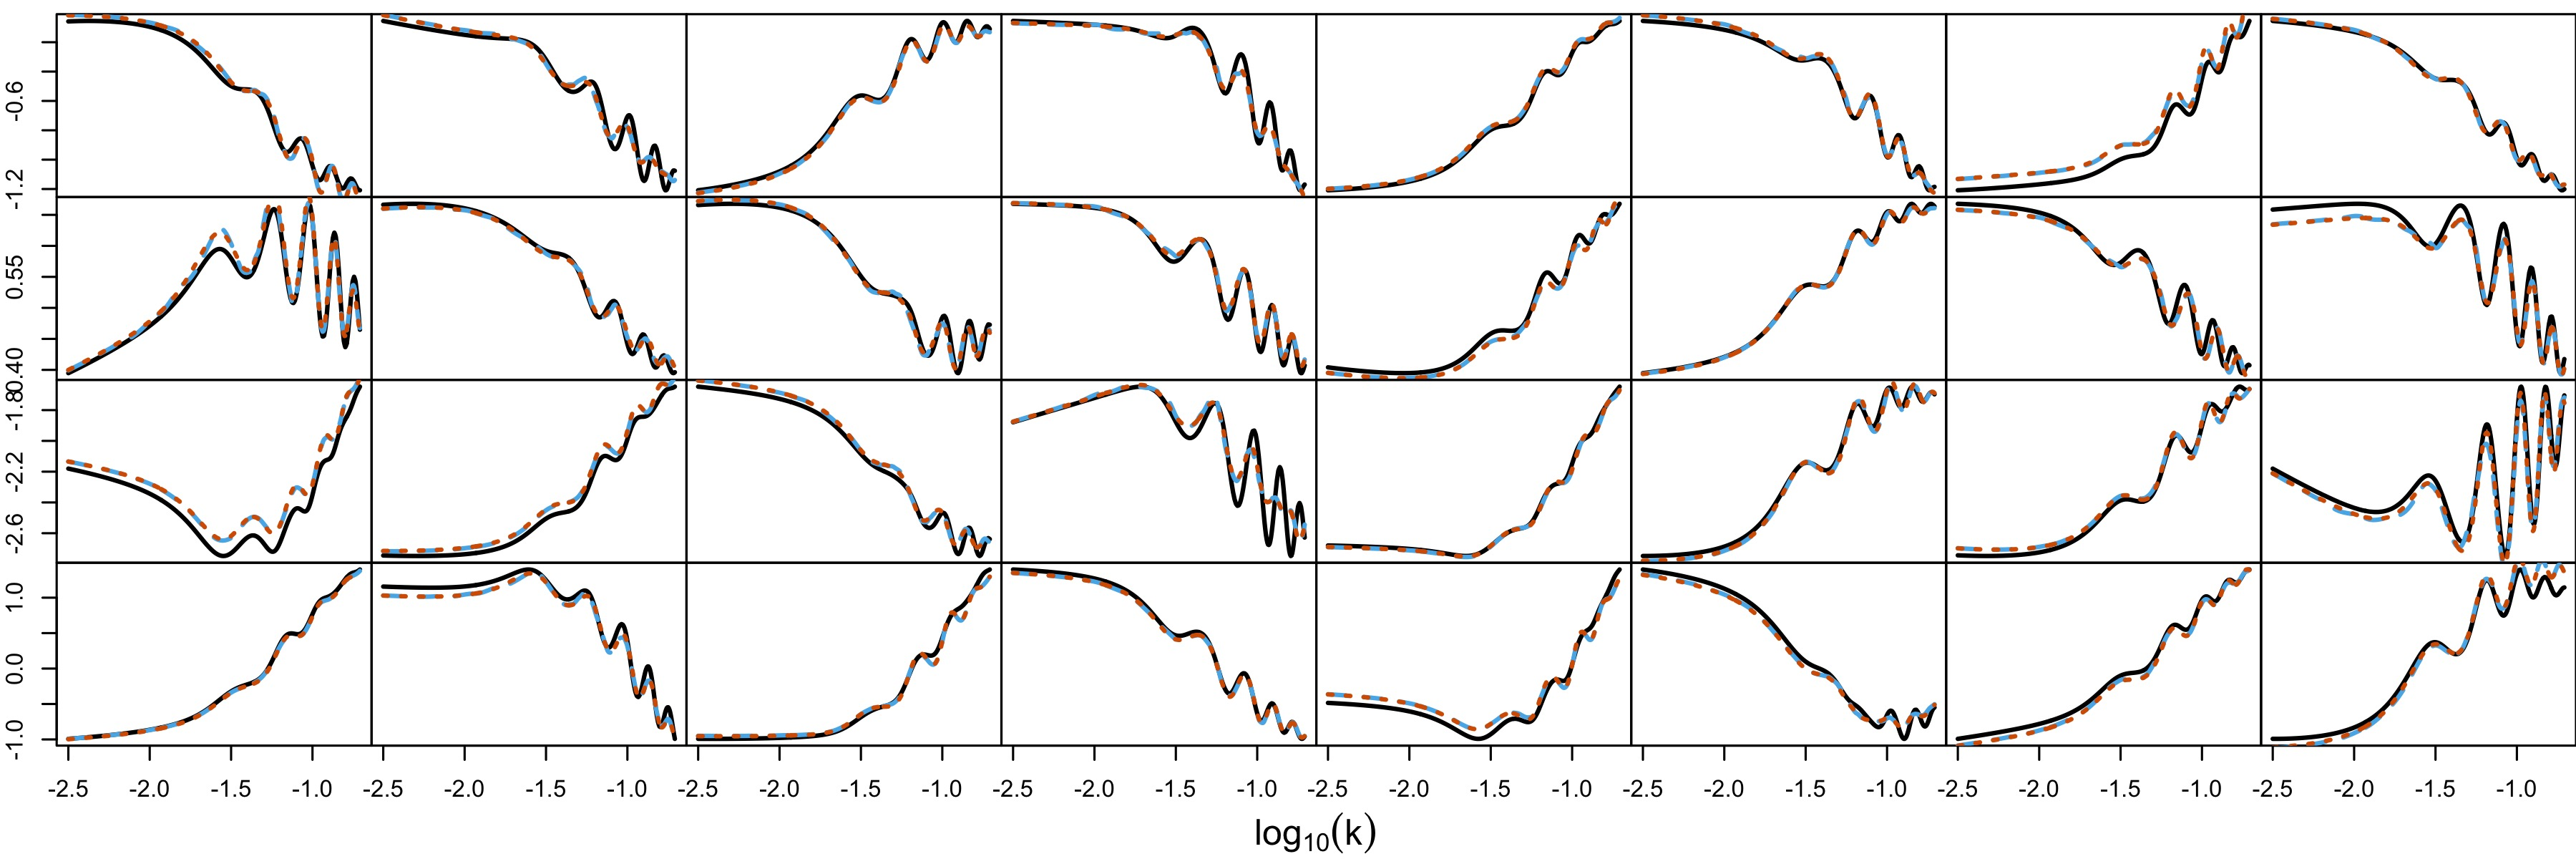
\includegraphics[width=0.85\textwidth]{pred_diffs_CAMB.jpeg}
    \caption{Predictions of power matter spectra for each of the 32 CAMB test cosmologies,
             after centering and scaling (to accentuate differences). 
             The true infinite resolution run is shown in black, the PC prediction 
             trained on the infinite resolution spectra is in dashed blue, and the PC prediction trained
             on the DGP.FCO posterior means is in dotted orange.}
    \label{fig:pca_preds_v_camb}
\end{figure}

Since CAMB offers the ``true'' infinite-resolution spectra, we have the opportunity to benchmark our
results in two ways.  First, we may compare our predictions to the true power spectrum for each held-out
cosmology.  Second, we may leverage the infinite-resolution spectra for the training cosmologies in
place of our estimated $\hat{S}_j$ from our DGP.FCO model, to get a sense of the ``best-case" predictions 
that could originate from the PC decomposition.  
Figure \ref{fig:pca_preds_v_camb} compares our predictions (DGP.FCO + PC, dotted orange)
to these ``best-case'' predictions (true + PC, dashed blue) and the actual true spectra (solid black)
for each of the 32 held-out test cosmologies.  
The agreement between our predictions and the ``best-case'' predictions indicates that DGP.FCO is effectively
capturing the true power matter spectra of the training cosmologies.
The high level of agreement between the pairs of predictions and the true spectra across cosmologies
indicates our PC model is providing effective predictions of held-out power spectra.
We then compare the mean squared errors of our predictions and the ``best-case'' 
predictions across all held-out cosmologies, with results shown in Figure \ref{fig:mse_camb}.  We again
see only minimal differences between the two, confirming that DGP.FCO is offering effective
estimates of the true spectra for each cosmology.

\begin{figure}
    \centering
    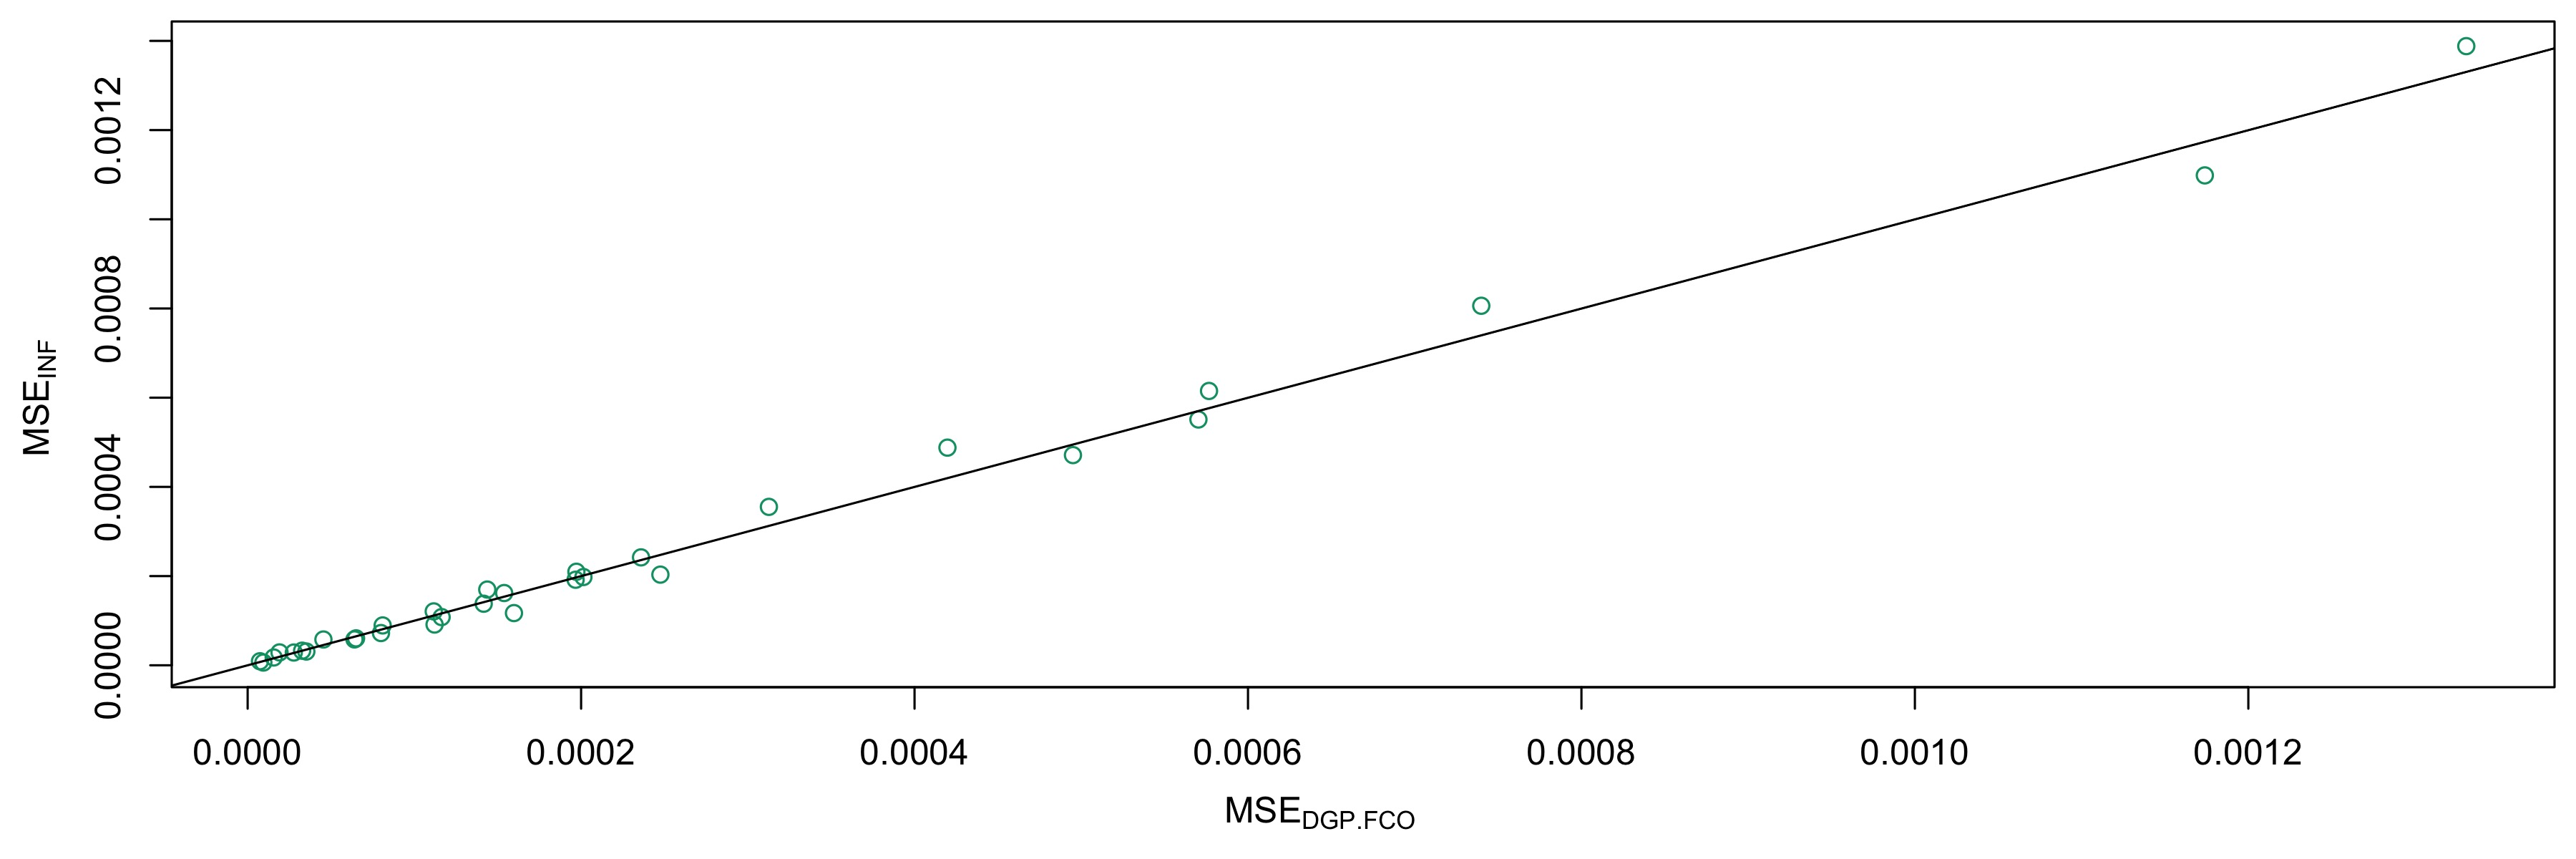
\includegraphics[width=\textwidth]{mse_dot.jpeg}
    \caption{Comparison of MSE for CAMB predictions, when training with DGP.FCO posterior 
             means and training with the ``true" infinite-resolution spectra. The identity line 
             provides equal MSE values amongst both methods.}   
    \label{fig:mse_camb}
\end{figure}

\subsection{Predicting Spectra for Mira-Titan}
\label{subsec:mira_pred}

Here we show prediction results for $N=6$ held-out cosmologies for the Mira-Titan dataset. 
We compare our method with Cosmic Emu \citep{moran2023mira}, the state-of-the-art emulator 
constructed on the same $m=111$ Mira-Titan cosmologies. Cosmic Emu uses a Bayesian approach 
where the ``true'' spectrum for each cosmology is modeled with a process convolution on Brownian motion. 
Nonstationarity is permitted through modeling the bandwidth parameter with a process 
convolution as well; this composition is referred to as a deep process convolution 
\citep[DPC;][]{moran2023mira}. Cosmic Emu also uses a principal components model to predict power matter 
spectra for held-out cosmologies as a function of $\psi$ \citep{gattiker2020sepia}.

Using our proposed DGP.FCO approach and Cosmic Emu, we obtain two sets of predictions for $\hat{S}_t(\psi_t)$ 
with $t\in\{1,\ldots,6\}$ indexing the six held-out cosmologies.  In this real-world example, we have
no ``truth" for the Mira-Titan hold-outs against which to benchmark. In an effort to assess the 
accuracy of these predictions, we also separately fit our DGP.FCO model on each of these testing cosmologies
(leveraging the perturbation theory, low resolution runs, and high resolution run to predict the underlying
power matter spectrum).  Although these predicted ``in-sample'' spectra are not formal ``truths,'' we find them to be
useful benchmarks for our ``out-of-sample'' predictions.  The individual predictions for each method and 
held-out cosmology are shown in Figure \ref{fig:plot_pred_1to6}, centered by the in-sample DGP.FCO
posterior means.  Predictions closer to zero represent a better fit. 

\begin{figure}[!b]
    \centering
    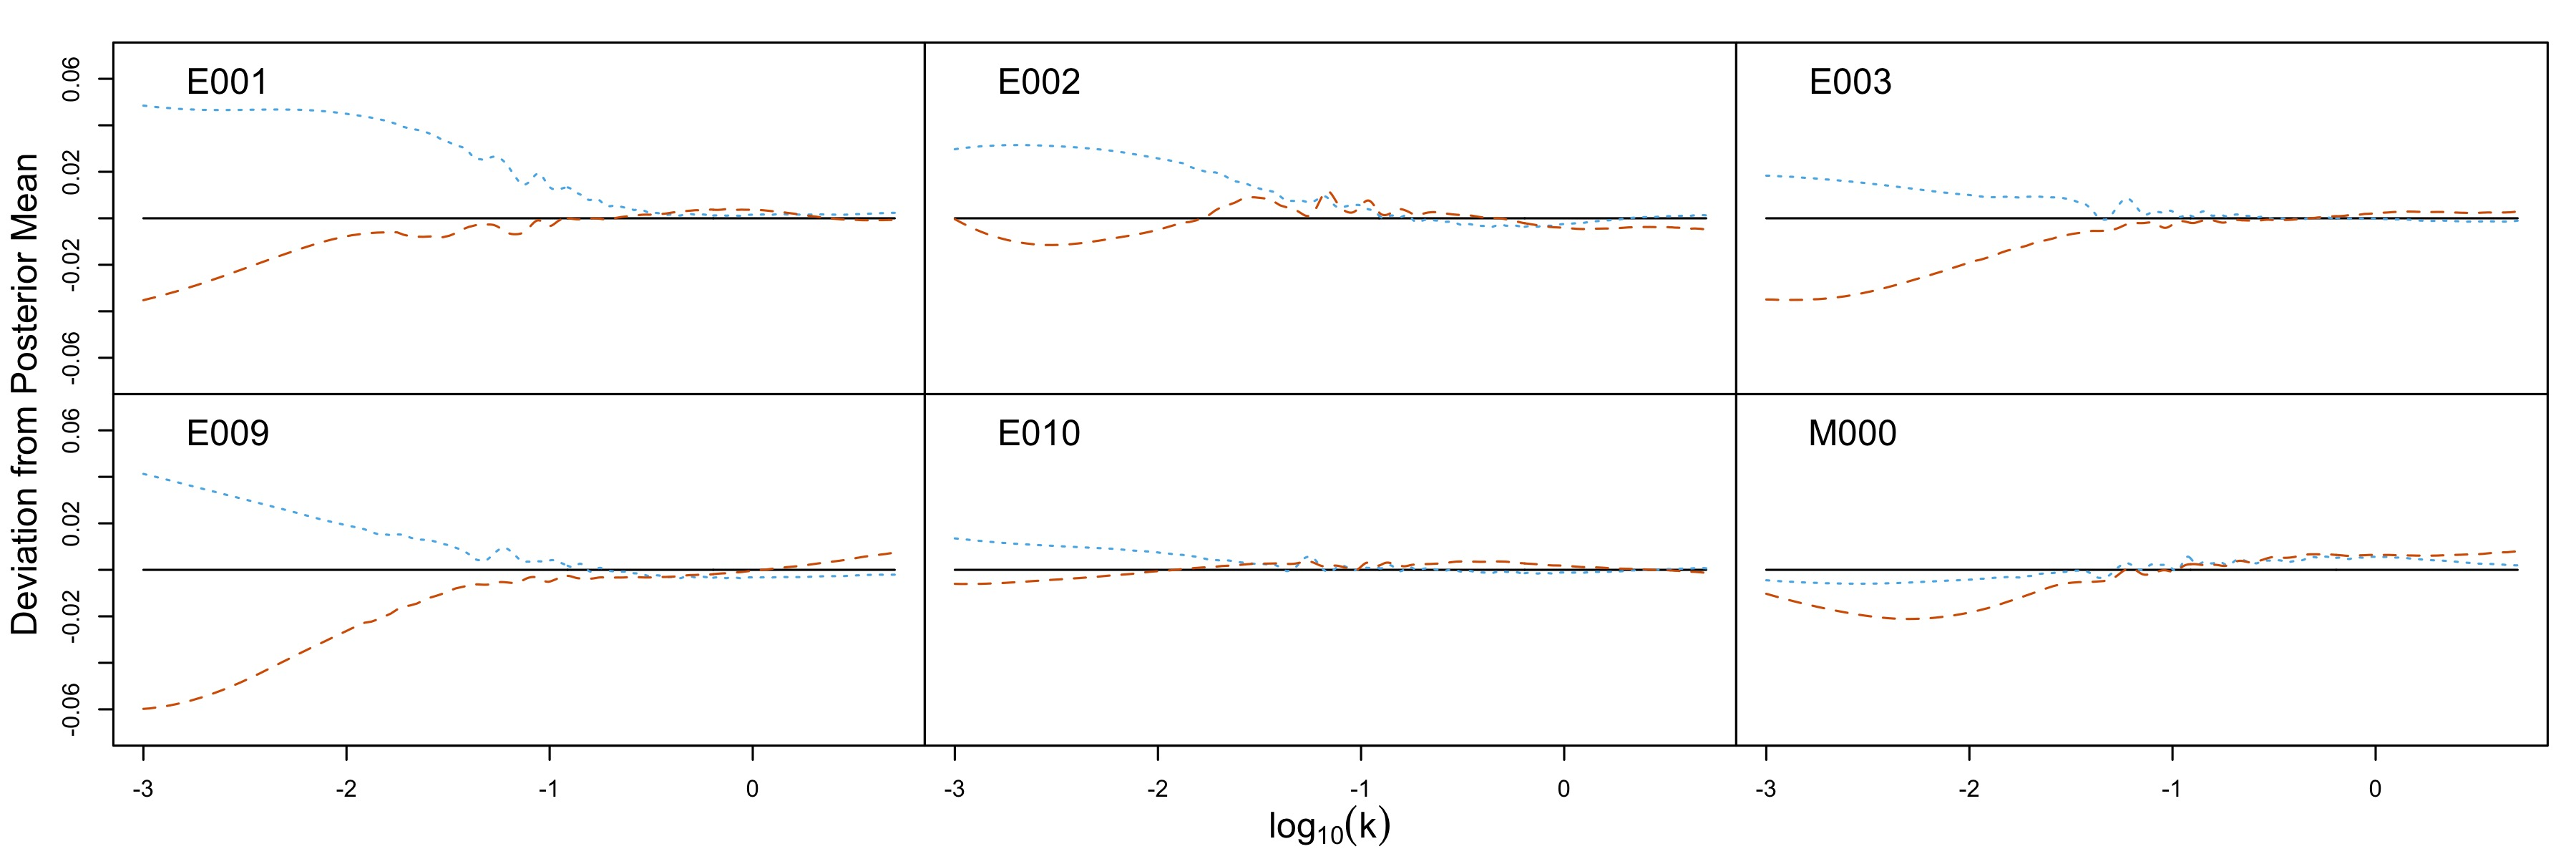
\includegraphics[width=\textwidth]{pred_1to6.jpeg}
    \caption{Results of all six predictions for both methods on the held-out 
    cosmologies (DGP.FCO posterior mean subtracted). CosmicEMU is dotted blue and DGP.FCO is dashed orange.
    Closer to the dotted zero line indicates a better fit with the DGP.FCO posterior mean.}
    \label{fig:plot_pred_1to6}
\end{figure}

From these predictions, we can calculate MSE against the in-sample DGP.FCO predictions across the 6
test cosmologies. 
Our out-of-sample DGP.FCO + PC prediction achieves the greatest reduction in MSE in the region 
where perturbation theory and the low-resolution runs are deemed unbiased (see Figure \ref{fig:mse_by_k}). 
For the region where only the high-resolution run is unbiased, Cosmic Emu has a marginally lower
MSE. Our MSE is lower at 55\% of $k$ values considered. These results indicate that DGP.FCO 
competes favorably with the state-of-the-art Cosmic Emu model.

\begin{figure}
    \centering
    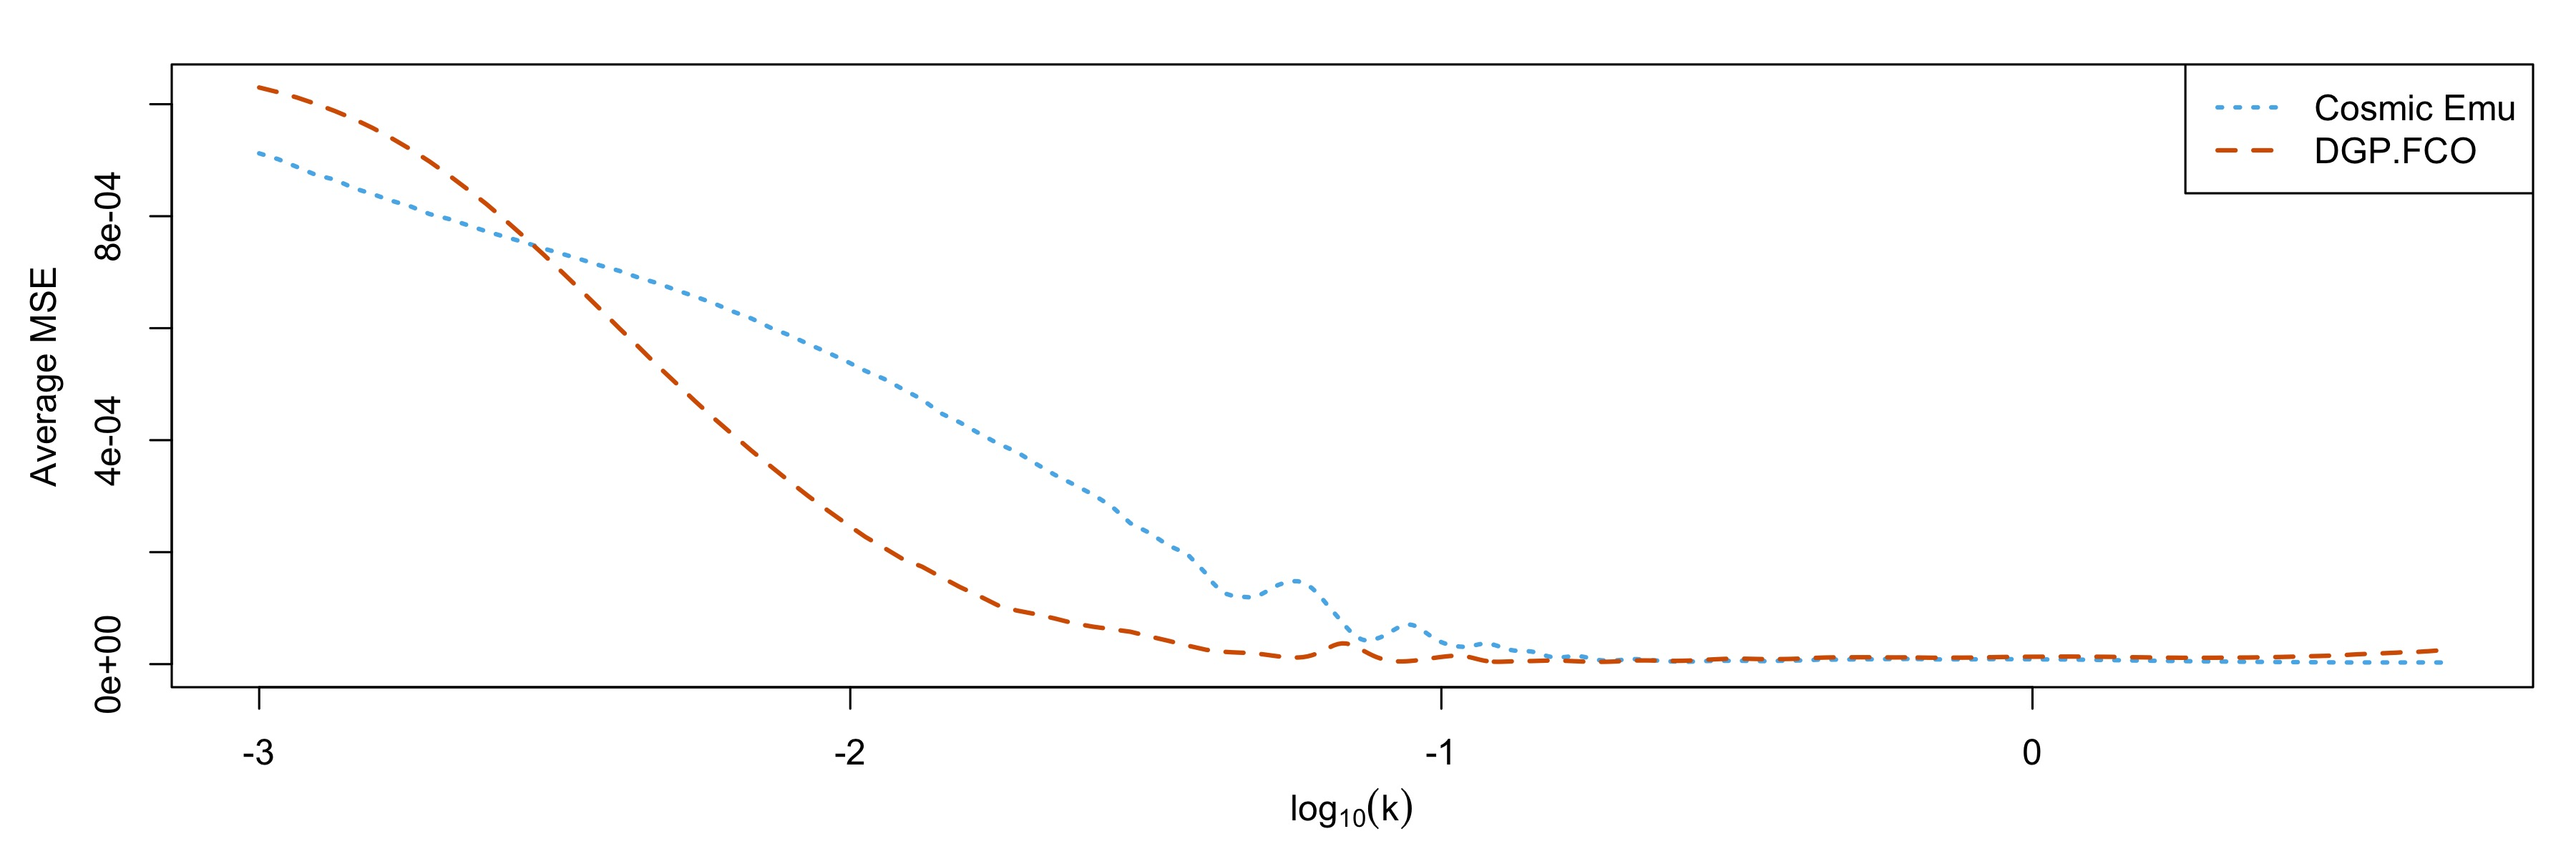
\includegraphics[width=\textwidth]{mse_by_k.jpeg}
    \caption{MSE across each of the 6 hold out cosmologies for each $k$ value. Cosmic Emu 
    performance is shown in dotted blue, and DGP.FCO performance is shown in dashed orange.}
    \label{fig:mse_by_k}
\end{figure}

\section{Discussion}
\label{sec:disc}

In this work, we introduced a novel Bayesian hierarchical framework that leverages deep 
Gaussian processes (DGPs) to model smooth latent functions from correlated functional outputs, 
such as those arising in cosmological simulations. Our model (DGP.FCO) builds on the 
compositional nature of DGPs and introduces an additional outer layer to explicitly 
model correlated observational errors within each spectrum. Through a simulation study, 
we demonstrated that DGP.FCO offers improved uncertainty 
quantification compared to existing methods.

We applied DGP.FCO to both the CAMB and Mira-Titan datasets, generating posterior mean estimates 
and predicting at held-out cosmological settings. Across both datasets, DGP.FCO 
consistently performs well against competitive baselines, showcasing strong generalization and 
flexibility in complex, functional data regimes.

Several avenues for future research arise. Beyond modeling dark matter power 
spectra, DGP.FCO could be extended to hydrodynamical simulation outputs in cosmology, which 
often share similar functional structures and error correlations. More broadly, this approach may be 
applicable in other scientific domains involving structured functional outputs, especially those 
with spatial or temporal dependencies.

In addition, generating predictions over large cosmological grids opens the door to detailed 
sensitivity analyses, enabling researchers to disentangle parameter interactions and identify 
the most influential physical drivers of the spectra. From a modeling standpoint, further 
developments could include joint modeling of latent layers across cosmologies, and extensions 
to redshifts beyond $z=0$. Lastly, a hybrid framework combining DGP.FCO with Cosmic Emu, leveraging 
the strengths of each at different scales of $k$, may yield more accurate predictions.

\section{Acknowledgments}
\label{sec:ack}

\textcolor{red}{This work was in part supported by the U.S. Department
of Energy, Office of Science, Office of Advanced Scientific Computing Research, 
Scientific Discovery through Advanced Computing (SciDAC) program through 
Grant 420453 "Enabling Cosmic Discoveries in the Exascale Era."}

The authors are pleased to acknowledge Advanced Research Computing at Virginia Tech 
(\url{https://arc.vt.edu/}) as well as the Shared Computing Cluster (SCC) administered
by Boston University's Research Computing Services (\url{www.bu.edu/tech/support/research/})
for providing computational resources and technical support that have contributed 
to the results reported within this paper.

\appendix
\renewcommand{\thesection}{Appendix \Alph{section}}

\section{Integrated Likelihood}
\label{sec:apdx_int_lik}
Here, we establish that under the model:

$$
\begin{aligned}
Y_i|S,W &\sim N\big(S, \Sigma_\varepsilon\big), \quad i \in \{1,\dots, r\}\\
S|W &\sim N\big(\boldsymbol{\mu}, \Sigma_S(w,w')\big)\\
W &\sim N\big(\mathbf{0}, \Sigma_W(x,x')\big) \\
\end{aligned}
$$

We can obtain the integrated likelihood $p(Y_i|W)=\int p(Y_i|S,W)p(S|W) dS$, 
with the following calculations:
$$
\begin{aligned}
p(Y_i|W) &= \int p(Y_i|S,W)p(S|W)dS \\
&\propto \int\exp\left(-\frac{1}{2} \left[Y_i^T\Sigma_\varepsilon^{-1} Y_i 
- 2Y_i^T\Sigma_\varepsilon^{-1} S + S^T \Sigma_\varepsilon^{-1} S + S^T \Sigma_S^{-1} S 
-2S^T \Sigma_S^{-1} \boldsymbol{\mu} 
+ \boldsymbol{\mu}^T \Sigma_S^{-1} \boldsymbol{\mu} \right]\right)dS \\
\end{aligned}
$$

If we focus only on terms containing $S$, we have 
$$
\begin{aligned}
    \exp\Big(-\frac{1}{2} \big[S^T &(\Sigma_\varepsilon^{-1}+\Sigma_S^{-1}) S 
    -2S^T (\Sigma_S^{-1} \boldsymbol{\mu} + \Sigma_\varepsilon^{-1} Y_i) \big]\Big) \\
&= \exp\left(-\frac{1}{2} \left[S^T (\Sigma_\varepsilon^{-1}+\Sigma_S^{-1}) S 
-2S^T (\Sigma_\varepsilon^{-1}+\Sigma_S^{-1})(\Sigma_\varepsilon^{-1}
+\Sigma_S^{-1})^{-1}(\Sigma_S^{-1} \boldsymbol{\mu} + \Sigma_\varepsilon^{-1} Y_i) \right]\right)
\end{aligned}
$$

To complete the square, we add and subtract $(\Sigma_S^{-1} \boldsymbol{\mu} 
+ \Sigma_\varepsilon^{-1} Y_i)^T(\Sigma_\varepsilon^{-1}+\Sigma_S^{-1})^{-1}
(\Sigma_S^{-1} \boldsymbol{\mu} + \Sigma_\varepsilon^{-1} Y_i)$, 
which then gives the kernel for $S \sim N\left((\Sigma_\varepsilon^{-1}
+\Sigma_S^{-1})^{-1}(\Sigma_S^{-1} \boldsymbol{\mu} + \Sigma_\varepsilon^{-1} Y_i), 
(\Sigma_\varepsilon^{-1}+\Sigma_S^{-1})^{-1} \right)$. 
This removes the integral and leaves us with the following terms for $Y_i|W$:
$$
\begin{aligned}
&\exp\Big(-\frac{1}{2}\big[Y_i^T\Sigma_\varepsilon^{-1} Y + 
\boldsymbol{\mu}^T\Sigma_S^{-1} \boldsymbol{\mu} - (\Sigma_S^{-1} \boldsymbol{\mu} + 
\Sigma_\varepsilon^{-1} Y_i)^T(\Sigma_\varepsilon^{-1}+\Sigma_S^{-1})^{-1} 
(\Sigma_S^{-1} \boldsymbol{\mu} + \Sigma_\varepsilon^{-1} Y_i)\big]\Big) \\
&= \exp\Big(-\frac{1}{2}\big[Y_i^T\big(\Sigma_\varepsilon^{-1} - 
\Sigma_\varepsilon^{-1}(\Sigma_\varepsilon^{-1}+\Sigma_S^{-1})^{-1}\Sigma_\varepsilon^{-1}\big)Y_i 
-2Y_i^T \Sigma_\varepsilon^{-1}(\Sigma_\varepsilon^{-1}+\Sigma_S^{-1})^{-1}\Sigma_S^{-1} \boldsymbol{\mu} \\
&\qquad \qquad \qquad + \boldsymbol{\mu}^T (\Sigma_S^{-1} - \Sigma_S^{-1}(\Sigma_\varepsilon^{-1}
+\Sigma_S^{-1})^{-1}\Sigma_S^{-1}) \boldsymbol{\mu}\big]\Big) \\
&= \exp\Big(-\frac{1}{2}\big((Y_i-\boldsymbol{\mu})^T(\Sigma_\varepsilon+\Sigma_S)^{-1}
(Y_i-\boldsymbol{\mu}) \big)\Big)
\end{aligned}
$$

With the last equality resulting from the use of the Sherman–Morrison–Woodbury formula, 
yielding $\big(\Sigma_\varepsilon^{-1} - \Sigma_\varepsilon^{-1}(\Sigma_\varepsilon^{-1}+
\Sigma_S^{-1})^{-1}\Sigma_\varepsilon^{-1} = (\Sigma_S^{-1} - \Sigma_S^{-1}
(\Sigma_\varepsilon^{-1}+\Sigma_S^{-1})^{-1}\Sigma_S^{-1}) = (\Sigma_\varepsilon+\Sigma_S)^{-1}$. 
We also use the fact that $\Sigma_\varepsilon^{-1}(\Sigma_\varepsilon^{-1}+
\Sigma_S^{-1})^{-1}\Sigma_S^{-1} = (\Sigma_\varepsilon + \Sigma_S)^{-1}$, 
which holds since it can be shown that 
$[\Sigma_S(\Sigma_\varepsilon^{-1}+\Sigma_S^{-1})\Sigma_\varepsilon](\Sigma_\varepsilon+\Sigma_S)
=(\Sigma_\varepsilon+\Sigma_S)(\Sigma_\varepsilon+\Sigma_S)$.

Therefore, we have that $Y_i|W \sim N\big(\boldsymbol{\mu}, \Sigma_S(w,w')+\Sigma_\varepsilon(w,w')\big)$.

\section{Conditional Distribution of Power Spectrum, Given Weighted Average}
\label{sec:apdx_SgivenY}

From our model specification, we have the following:

\[
S \sim \mathcal{N}(\boldsymbol{\mu}, \Sigma_S)
\]
\[
\bar{Y} \mid S \sim \mathcal{N}(S, \Sigma_\epsilon)
\]

Then, to find the distribution of $S|\bar{Y}$, we apply Bayes' Theorem below, 
where $\propto$ indicates proportionality:
\[
P(S \mid \bar{Y}) \propto P(\bar{Y} \mid S) P(S)
\]

\[
\propto \exp\left(-\tfrac{1}{2} (\bar{Y} - S)^T \Sigma_\epsilon^{-1} (\bar{Y} - S) \right) 
\cdot \exp\left(-\tfrac{1}{2} (S - \boldsymbol{\mu})^T \Sigma_S^{-1} (S - \boldsymbol{\mu})\right)
\]

\[
\propto \exp\left(-\tfrac{1}{2} \left[ \bar{Y}^T \Sigma_\epsilon^{-1} \bar{Y} 
- 2 S^T \Sigma_\epsilon^{-1} \bar{Y} + S^T \Sigma_\epsilon^{-1} S + S^T \Sigma_S^{-1} S 
- 2 S^T \Sigma_S^{-1} \boldsymbol{\mu} + \boldsymbol{\mu}^T \Sigma_S^{-1} \boldsymbol{\mu} \right] \right)
\]

\[
\propto \exp\left( -\tfrac{1}{2} \left[ S^T (\Sigma_\epsilon^{-1} + \Sigma_S^{-1}) S 
- 2 S^T (\Sigma_\epsilon^{-1} \bar{Y} + \Sigma_S^{-1} \boldsymbol{\mu}) \right] \right)
\]

From properties of the multivariate normal distribution \citep[e.g., Equation 7.1 of][]{hoff2009first},
we can establish that the mean and covariance of $S|\bar{Y}$ will be $\boldsymbol{m}$
and $C$ respectively, where we can solve for these values with:

\[
C^{-1} = \Sigma_\epsilon^{-1} + \Sigma_S^{-1}
\]
\[
C^{-1} \boldsymbol{m} = \Sigma_\epsilon^{-1} \bar{Y} + \Sigma_S^{-1} \boldsymbol{\mu}
\]

Then,
\[
C = (\Sigma_\epsilon^{-1} + \Sigma_S^{-1})^{-1}
\]
\[
\boldsymbol{m} = \left( \Sigma_S^{-1} + \Sigma_\epsilon^{-1} \right)^{-1} 
\left( \Sigma_\epsilon^{-1} \bar{Y} + \Sigma_S^{-1} \boldsymbol{\mu} \right)
= C \cdot \left( \Sigma_\epsilon^{-1} \bar{Y} + \Sigma_S^{-1} \boldsymbol{\mu} \right)
\]

Therefore, we have the result that $S|\bar{Y} \sim \mathcal{N}(\boldsymbol{m}, C)$.

\section{Simulation Study Additional Results}
\label{sec:apdx_sims}

\begin{figure}[H]
    \centering
    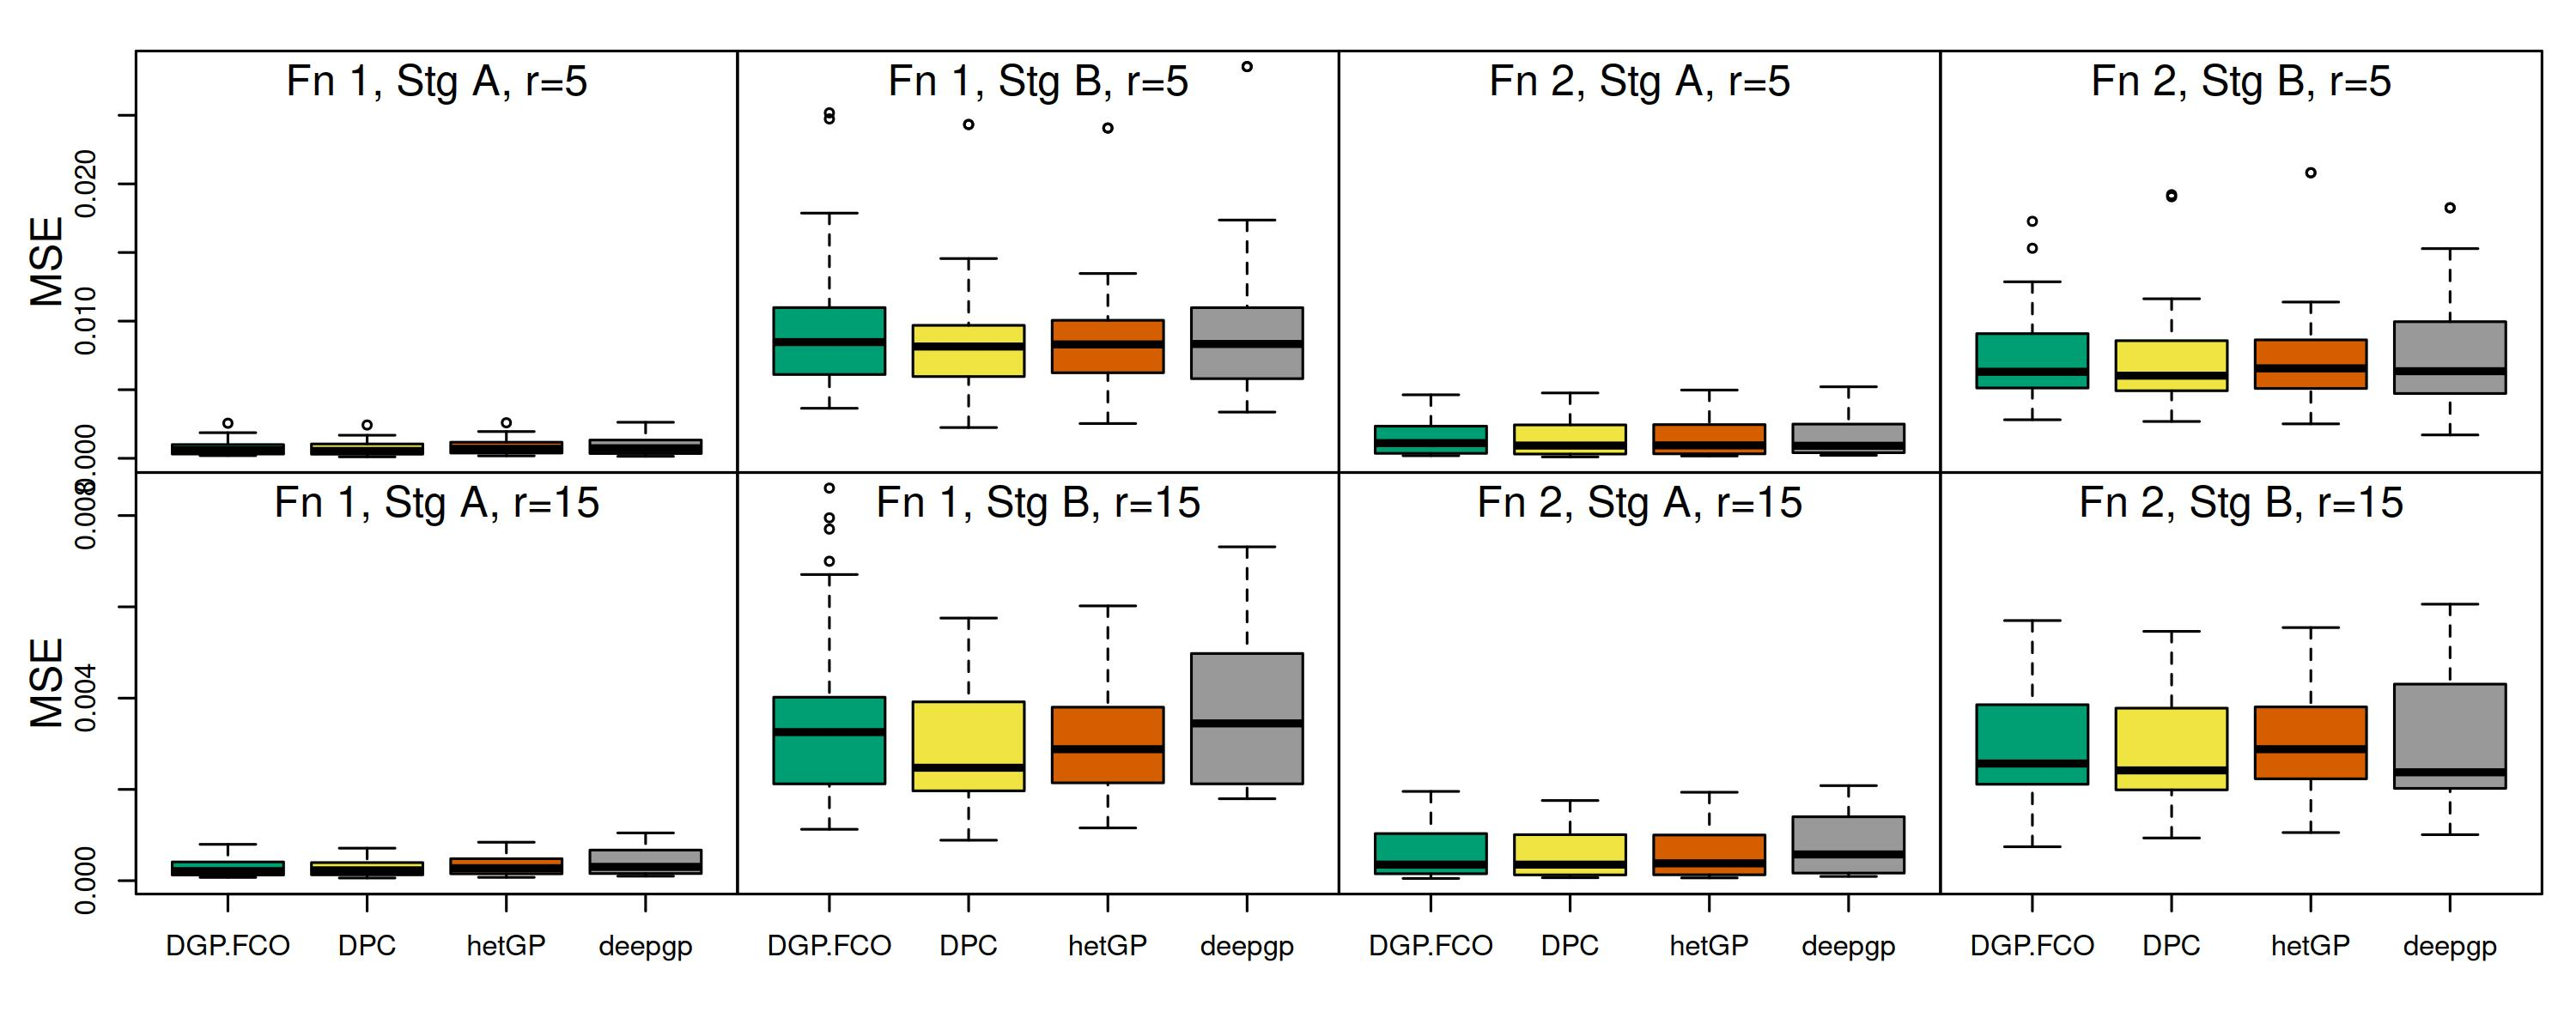
\includegraphics[width=\textwidth]{sims_MSE.jpeg}
    \caption{Boxplot of MSEs across two different functions and covariance settings 
             (lower is better). For each case, the boxplot is constructed from 20 
             random batches were simulated. Each column represents a function/variance 
             specification pair, and each row shows results for batch sizes of 
             either 5 (top) or 15 (bottom).}    
    \label{fig:sims_MSE}
\end{figure}

\section{Details on Basis Decomposition for Predictions}
\label{sec:apdx_basis}

Here, we begin with a $n \times m$ matrix composed of $m$ posterior means, 
each of length $n$, denoted by $\boldsymbol\eta$. To facilitate more efficient estimation, 
we use singular value decomposition \citep[SVD; e.g.,][]{banerjee2014linear}, 
where $\boldsymbol\eta = UDV^T$; $U$ and $V$ are orthogonal matrices of size $n \times n$ 
and $m\times m$, respectively. $D$ is a diagonal matrix containing the singular values. 
Here, $\boldsymbol\eta$ has rank $r=\text{min}\{m,n\}$ (for our applications, $r=111$ for Mira-Titan 
and $r=32$ for CAMB), which determines the number of non-zero elements in $D$. We find an alternative 
decomposition where $\Sigma$ is a diagonal matrix with the non-zero singular values of 
$\boldsymbol\eta$, and $U_1$ and $V_1$ are matrices with orthonormal columns of size 
$n_\eta \times r$ and $m \times r$, respectively. 

Following \cite{higdon2008computer, higdon2010estcosmo}, we equivalently decompose 
$\boldsymbol\eta$ into a principal component (PC) basis matrix 
$B^* = \frac{1}{\sqrt{m}}U_1\Sigma$ along with its corresponding weights 
$\Gamma^* = \sqrt{m}V_1$. Without loss of generality, we can perform this decomposition 
after an overall mean trend is removed. If we use $p_\eta < r$ PCs, this will reduce 
$B$ and $\Gamma$ to be the first $p_\eta$ columns of $B^*$ and $\Gamma^*$ respectively and 
result in an approximation where 

\begin{equation}
    \boldsymbol\eta= UDV^T = U_1\Sigma V_1^T \approx B\Gamma^T.
\end{equation}

\bibliographystyle{jasa}
\bibliography{references}

\end{document}
